\documentclass{book}
\usepackage{amsmath, amsthm, graphicx, amsfonts, float, bm}
\usepackage[english]{babel}
\graphicspath{ {./images/} }

\usepackage{geometry}
 \geometry{
 a4paper,
 total={170mm,237mm},
 left=20mm,
 top=30mm,
 }
 \usepackage[hidelinks]{hyperref}

\newcommand\at[2]{\left.#1\right|_{#2}}
\DeclareMathOperator{\sgn}{sgn}
\DeclareMathOperator{\spec}{spec}
\DeclareMathOperator{\vspan}{span}
\DeclareMathOperator{\col}{col}
\DeclareMathOperator{\des}{des}
\DeclareMathOperator*{\argmax}{arg\,max}
\DeclareMathOperator*{\argmin}{arg\,min}
\newcommand{\notimplies}{%
  \mathrel{{\ooalign{\hidewidth$\not\phantom{=}$\hidewidth\cr$\implies$}}}}
\newcommand{\R}{\mathbb{R}}
\newcommand{\N}{\mathbb{N}}
\newcommand{\deriv}[1]{\displaystyle\frac{d}{d #1}}
\newcommand{\traj}{(\bar{\mathbf{x}},\bar{\mathbf{u}})}
\newcommand{\fatone}{\boldsymbol{1}}
\newcommand{\fatl}{\boldsymbol{\ell}}

\newtheoremstyle{theoremv2}{}{}{}{}{\bfseries}{}{\newline}{}
\theoremstyle{theoremv2}
\newtheorem{theorem}{Theorem}[chapter]
\newtheorem{proposition}{Proposition}[chapter]
\newtheoremstyle{defv2}{}{}{}{}{\bfseries}{}{\newline}{}
\theoremstyle{defv2}
\newtheorem{definition}{Definition}[chapter]
\theoremstyle{remark}
\newtheorem*{remark}{Remark}
\theoremstyle{remark}
\newtheorem*{notation}{Notation}
\theoremstyle{definition}
\newtheorem*{lemma}{Lemma}
\theoremstyle{definition}
\newtheorem*{corollary}{Corollary}

\title{Distributed Autonomous Systems M}
\author{Dante Piotto}
\date{spring semester 2024}


\begin{document}
\maketitle
\tableofcontents

\chapter{Introduction and scenarios}
\section{Distributed Autonomous System}
Each agent $i\in\{1,\dots,N\}$ has 
\begin{itemize}
    \item local physical and/or cyber state $x_i$
    \item computational and sensing capabilities
    \item communication capability: exchange messages with "neighbours"
\end{itemize}


\section{Scenarios and applications of distributed systems}
\begin{itemize}
    \item Averaging: distributed estimation, opinion dynamics
    \item Distrbuted control in cooperative robotics
    \item Distributed optimization 
        \begin{itemize}
            \item distributed machine learning
            \item distributed decision-making in cooperative robotics
            \item distributed optimal control in energy systems and cooperative robotics
        \end{itemize}
\end{itemize}


\section{Measurement filtering in wireless sensor networks}
Consider a network of $N$ sensors with local sensing, computation and communication. Agent $i,i\in\{1,\dots,N\}$, takes a local measurement from the environment (temperature, pressure, etc.). Let $x_{i0}\in\R$ be the scalar local measurement
Agents are interested in agreeing on the average of the measurements, 
\[
    x_{\text{avg}}=\displaystyle\frac{1}{N}\displaystyle\sum_{i=1}^{N}x_{i0}
\]
to have a better estimate of the environment quantity

Consider the following "distributed algorithm" based on "local" linear averaging, for each $i\in\{1,\dots,N\}$
\begin{gather*}
    x_i^0=x_{i0}\\
    x_i^{k+1} = \text{average}(x_i^k,\{x_j^k,j\text{ "neighbour" of }i\}), \qquad k\in\N
\end{gather*}
generalizing coefficients of the update: 
\begin{gather*}
    x_i^0=x_{i0}\\
    x_i^{k+1} = \displaystyle\sum_{j=1}^{N} a_{ij}x_j^k \qquad k\in\N
\end{gather*}
\begin{remark}
    $a_{ij}\geq 0$ and $\sum_{j=1}^{N}a_{ij}=1$
\end{remark}
\begin{remark}
    $a_{ij}=0$, for some $j\in\{1,\dots,N\}$, i.e. $a_{ij}=0$ if $i$ does not have access to the estimate of $j$
\end{remark}


\section{Parameter Estimation in Wireless Sensor Networks}

Consider a network of $N$ sensors with local sensing, computation and communication aiming at estimating a common parameter $\theta^*\in\R$
Each sensor $i$ measures 
\[
    y_i=B_i\theta^* + v_i
\]
with $y_i\in\R^{m_1},B_i$ known matrix and $v_i$ a random measurement noise. Assume $v_1,\dots,v_N$ independent and Gaussian, with zero mean and covariance $E[v_iv_i^T]=\Sigma_i$. Assume $\sum_{i=1}^{N}m_i\geq m$ and $\begin{bmatrix}
    B_1 \\ \vdots \\ B_N
\end{bmatrix} $ full rank
Compute a least-squares estimate 
\[
    \hat\theta = \argmin_\theta \displaystyle\sum_{i=1}^{N}(y_i-B_i\theta)^T\Sigma_i^{-1}(y_i-B_i\theta)
\]
The optimal solution is 
\begin{align*}
    \hat\theta &= \left(\displaystyle\sum_{i=1}^{N}B_i^T\Sigma_i^{-1}B_i \right)^{-1} \displaystyle\sum_{i=1}^{N}B_i^T\Sigma_i^{-1}y_i\\ 
    & =  \left(\displaystyle\frac{1}{N}\displaystyle\sum_{i=1}^{N}B_i^T\Sigma_i^{-1}B_i \right)^{-1} \displaystyle\frac{1}{N}\displaystyle\sum_{i=1}^{N}B_i^T\Sigma_i^{-1}y_i\\ 
\end{align*}
The optimal solution can be obtained by computing two averages $\frac{1}{N}\displaystyle\sum_{i=1}^{N}\beta_i$ and $\frac{1}{N}\displaystyle\sum_{i=1}^{N}\beta_i$

\subsection{Opinion Dynamics in Social Influence Networks}
Group of $N$ individuals, with $x_i^k$ being the opinion of individual $i$ at time $k$. Opinions are updated according to 
\[
    x_i^{k+1} = \displaystyle\sum_{j=1}^{N}a_{ij}x_j^k
\]


\section{Main questions in averaging algorithms}
\begin{itemize}
    \item Do node estimates converge? Do they converge to a common value ("reach consensus")?
    \item Do they reach consensus to the average ("average consensus")?
    \item How can we model communication  in general networks?
    \item Can we answer the above questions for general networks and communication protocols?
    \item What assumptions do we need on the communication network?
\end{itemize}

\section{Distributed control in cooperative robotics}
Team of $N$ (mobile) robots aiming to execute complex tasks
\subsubsection{Basic tasks}
\begin{itemize}
    \item rendevous, containment
    \item formation, flocking
    \item coverage
\end{itemize}
\subsubsection{Complex tasks}
\begin{itemize}
    \item pickup and delivery
    \item surveillance and patrolling
    \item exploration
    \item satellite constellation
\end{itemize}
\subsection{Main questions in cooperative robotics}
\begin{itemize}
    \item Do robot states asymptotically converge? 
    \item Do the asympototic staes satisfy the global, desired task?
    \item How can we model communication in (general) robotic networks?
    \item What assumptions do we need on the communication network?
    \item Can we answer the above questions for general networks and communication protocols?
\end{itemize}
\subsection{Distributed optimal control}
\begin{align*}
    \min_{\substack{x_1,\dots,x_N \\ u_1,\dots,u_N}} & \displaystyle\sum_{i=1}^{N}(\displaystyle\sum_{\tau=0}^{T-1}\ell_i(z_{i,\tau},u_{i,\tau})+m_i(z_{i,T}))\\
    \text{subj to} & \displaystyle\sum_{i=1}^{N}H_iz_{i,\tau}\leq h, && \tau\in[0,T]\\ 
    & z_{i,\tau+1}=A_iz_{i,\tau}+B_iu_{i,\tau} && \forall i, \tau \in [0,T]\\ 
    & z_{i,\tau}\in Z_i, \quad u_{i,\tau}\in U_i, && \forall i, \tau \in [0,T]\\ 
\end{align*}









\chapter{Preliminaries on Algebraic Graph Theory}
\begin{definition}[Digraph]
    A digraph is a pair $G=(I,E)$ where $I={1,\dots,N}$ is a set of elements called \emph{nodes} and $E\subset I \times I$ is a set of ordered node pairs called \emph{edges}\\
    \emph{Edge}: the pair $(i,j)$ denotes an edge from $i$ to $j$\\ 
    \emph{Self-loop}: edge from a node to itself, i.e. $(i,i)$
\end{definition}
\begin{definition}[Undirected (di)graph]
    if for any $(i,j)\in E$ then $(j,i)\in E$  
\end{definition}
\begin{definition}[Subgraph]
    $(I',E')$ subgraph of $(I,E)$ if $I'\subset I$ and $E' \subset E$. Spanning subgraph if $I'=I$
\end{definition}
\begin{definition}[In-neighbours of $i$]$j\in I$ is an in-neighbour of $i\in I$ if $(j,i)\in E$
\end{definition}
\begin{definition}[Set of in-neighbours of $i$]
    $\mathcal{N}_i^{\text{IN}}=\{j\in\{1,\dots,N\}|(j,i)\in E\}$
\end{definition}
\begin{definition}[Out-neighbours of $i$]$j\in I$ is an out-neighbour of $i\in I$ if $(i,j)\in E$
\end{definition}
\begin{definition}[Set of out-neighbours of $i$]
    $\mathcal{N}_i^{\text{IN}}=\{j\in\{1,\dots,N\}|(i,j)\in E\}$
\end{definition}
\begin{definition}[In-degree $\deg_i^{\text{IN}}$]
    number of in-neighbours, i.e. carinality of $\mathcal{N}_i^{\text{IN}}(\deg_i^{\text{IN}}=|\mathcal{N}_i^{\text{IN}}|)$

    Out-degree analogous
\end{definition}
\begin{definition}[Balanced digraph]
    A digraph $G$ is balanced if $\deg_i^{\text{IN}}=\deg_i^{\text{OUT}}$ for all $i\in\{1,\dots,N\}$
\end{definition}
\begin{definition}[Directed path]
    ordered sequence of nodes s.t. any pair of consecutive nodes is a directed edge. A path is \emph{simple} if no node appears more than once
\end{definition}
\begin{definition}[Directed cycle]
    simple directed path that starts and ends at the same node. Cycles of length one are called self-loops. Acyclic digraph if there are no cycles.
\end{definition}
\begin{definition}[Directed tree]
    Acyclic digraph s.t. there exists a node, root, s.t. any node can be reached by only one directed path starting at the root.
\end{definition}
\begin{definition}[Spanning tree]
    a spanning subgraph that is a (directed) tree
\end{definition}
\begin{definition}[Periodic graph]
    if there exists a $k>1$ period, that divides the length of every cycle.
\end{definition}
Note: a graph with self-loops is aperiodic.
\begin{definition}[Strongly connected digraph]
    if there exists a directed path from any node to any other node
\end{definition}
\begin{definition}[Connected undirected graph]
    if there exists a path from any node to any other node
\end{definition}
\begin{definition}[Globally reachable node]
    if one of its nodes can be reached from any other node by traversing a directed path
\end{definition}
\begin{definition}[Complete graph]
    Unweighted graph such that $\forall i,j\ \exists \ (i,j),\ (j,i) \in E$
\end{definition}
\begin{definition}[Weighted digraph]
    triplet $G=(I,E,\{a_{(i,j)}\}_{(i,j)\in E})$, where $(I,E)$ is a digraph and each $a_(i,j)$ is a strictly positive weight for the edge $(i,j)$
\end{definition}
\begin{definition}[Weighted in-degree]
    $\deg_i^\text{IN} = \displaystyle\sum_{j=1}^{N}a_{ji}$
\end{definition}
\begin{definition}[Weighted out-degree]
    $\deg_i^\text{OUT} = \displaystyle\sum_{j=1}^{N}a_{ij}$
\end{definition}
A graph is said to be weight balanced if $\deg_i^\text{IN} = \deg_i^\text{OUT}$ for all nodes $i\in\{1,\dots,N\}$
\begin{definition}[Weighted adjacency matrix]
    non-negative matrix $A$ s.t. the entry $(i,j)$ of $A$, denoted $a_{ij}$, satisfies:
    \begin{itemize}
        \item $a_{ij} > 0$ if $(i,j)\in E$
        \item $a_{ij} = 0$ otherwise
    \end{itemize}
\end{definition}
\begin{definition}[Adjacency matrix]
    matrix $A$ with entries $a_{ij}=1$ if $(i,j)\in E$ and $a_{ij}=0$ otherwise
\end{definition}
\begin{definition}[Weighted in/out degree]
    $\deg_i^\text{IN} = \displaystyle\sum_{j=1}^{N} a_{ji}$ and $\deg_i^\text{OUT} = \displaystyle\sum_{j=1}^{N} a_{ij}$
\end{definition}
\begin{definition}[Laplacian matrix]
    $L = D^\text{OUT} - A$
\end{definition}

\chapter{Averaging Systems}
\section{Distributed algorithm}
Given a network of $N$ agents communicating according to a fixed digraph $G$, i.e. each agent $i$ can receive messages only from in-neighbours in the graph, i.e. from $j\in\mathcal{N}_i^{\text{IN}}$. 
We start by considering a fixed graph, thus, each agent communicates with the same neighbours at each iteration $k\in\N$
\[
    x_i^{k+1}=\text{stf}_i(x_i^k,\{x_j^k\}_{j\in\mathcal{N}_i^{\text{IN}}}), \qquad i\in\{1,\dots,N\}
\]
where $\text{stf}_i$ is a function depending only on state $x_i$ and states $x_j,j\in\mathcal{N}_i^{\text{IN}}$.

Alternative version with out-neighbours:
\[
    x_i^{k+1}=\text{stf}_i(\{x_j\}_{j\in\mathcal{N}_i^{\text{OUT}}})
\]
\section{Discrete-time averaging systems}
Let $G^{\text{comm}}=(I,E)$ be a fixed (communication) digraph (self loops included). A linear averaging distributed algorithm can be written as:
\[
    x_i^{k+1}=\displaystyle\sum_{J\in\mathcal{N}_i^{\text{IN}}}a_{ij}x_j^k \qquad i\in\{1\dots,N\}
\]
where $x_i^k\in\R$ is the state of agent $i$ at $k$ and $a_{ij}>0$ are positive weights. 
\begin{remark}
    The weights $a_{ij}$ are defined only for $(i,j)\in E$
\end{remark}
Wach $i$ uses only the states of neighbours $j\in\mathcal{N}_i^{\text{IN}}$, thus distributed algorithm.

For analysis purposes, let us define weights $a_{ij}=0$ for $(j,i)\notin E$. Thus we can rewrite the distributed algorithm as 
\[
    x_i^{k+1}=\displaystyle\sum_{j=1}^{N}a_{ij}x_j^k \qquad i\in\{1,\dots,N\}
\]
This is a LTI autonomous system 
\[
    \begin{bmatrix}
        x_1^{k+1}\\ \vdots \\ x_N^{k+1}
    \end{bmatrix} = \begin{bmatrix}
        a_{11} & \cdots & a_{1N} \\ 
        \vdots & \ddots & \vdots \\
        a_{N1} & \cdots & a_{NN}
    \end{bmatrix} \begin{bmatrix}
        x_1^k \\ \vdots \\ x_N^k
    \end{bmatrix}
\]
Which can be compactly written as  
\[
    x^{k+1} 0 Ax^k
\]
\begin{remark}
    The matrix A can be seen as the weighted adjacency matrix of the reverse digraph $G^{\text{comm,rev}}$ of the digraph $G^{\text{comm}}$
\end{remark}
If instead of in-neighbours we use out-neighbours, we call the digraph a sensing digraph $G^{\text{sens}}$. In this case the notation becomes consistent with graph theory, so we get 
\[
    x^{k+1} = A x^k
\]
where $A$ can be seen as the weighted adjacency matrix of the sensing digraph $G^{\text{sens}}$

\section{Stochastic matrices}
The non-negative square matrix $A\in\R^{N\times N}$ is 
\begin{itemize}
    \item row stochastic if $A\mathbf{1}=\mathbf{1}$ (each row sums to 1)
    \item column stochastic if $A^\top \mathbf{1}=\mathbf{1}$ (each column sums to 1)
    \item doubly stochastic if both row and column stochastic.
\end{itemize}
\begin{lemma}
    Let $A$ be a row-stochastic matrix and $G$ the associate digraph. If $G$ is strongly connected and aperiodic, then 
    \begin{enumerate}
        \item the eigenvalue $\lambda=1$ is simple; 
        \item all the other eigenvalues $\mu$ satisfy $|\mu|<1$
    \end{enumerate}
\end{lemma}
\begin{remark}
    The condition "$G$ contains a globally reachable node and the subgraph of globally reachable noes is aperiodic" is necessary and sufficient
\end{remark}
\begin{theorem}[Consensus]
    Consider a (discrete-time) averaging system with associated digraph $G$ and wieghted adjacency matrix $A$. Assume $G$ is strongly connected and aperiodic, and $A$ is row stochastic. Then 
    \begin{enumerate}
        \item there exists a left eigenvector $w\in\R^N,w>0$ (i.e. with positive components $w_i>0$ for all $i=1,\dots,N$) such that 
            \[
                \lim_{k\to\infty}x^k = \mathbf{1}\displaystyle\frac{w^\top x^0}{w^\top \mathbf{1}} = \begin{bmatrix}
                    1 \\ \vdots \\ 1
                \end{bmatrix} \displaystyle\frac{\sum_{i=1}^{N}w_ix_i^0}{\sum_{i=1}^{N}w_i}
            \]
            i.e., consensus is reached to $ \displaystyle\frac{\sum_{i=1}^{N}w_ix_i^0}{\sum_{i=1}^{N}w_i}$
        \item if additionally $A$ is doubly stochastic, then 
            \[
                \lim_{k\to\infty}x^k = \begin{bmatrix}
                    1 \\ \vdots \\ 1
                \end{bmatrix} \displaystyle\frac{\sum_{i=1}^{N}x_i^0}{N}
            \]
            i.e., average consensus is reached
    \end{enumerate}
\end{theorem}

\section{Example: Metropolis-Hastings weights}
Given an undirected unweighted graph $G$ with edge set $E$ and degrees $d_1,\dots,d_n$
\[
    a_{ij} = \begin{cases}
        \displaystyle\frac{1}{1+\max\{d_i,d_j\}} & \text{if } (i,j)\in E \text{ and } i\neq j\\
        1- \displaystyle\sum_{h\in\mathcal{N}_i \backslash \{i\}}^{} a_{ih} & \text{if } i=j\\ 
        0 & \text{otherwise}
    \end{cases}
\]
Result: the matrix $A$ is symmetric and doubly-stochastic.

\section{Time-varying digraphs}
A time-varying digraph is a sequence of digraphs $\{G(k)\}_{k\geq 0}$.
\begin{remark}
    The main definitions of in/out neighbours, in/out degree, adjacency matrix can be generalized by considering time-varying versions, i.e. $\mathcal{N}_i^{\text{IN}}(k)$, $\mathcal{N}_i^{\text{OUT}}(k)$, $\deg_i^{\text{IN}}(k)$ ,$\deg_i^{\text{OUT}}(k)$, $A(k)$ associated to each graph $G(k)$. Connectivity requires new definitions as assuming each $G(k)$ to be connected is too conservative.
\end{remark}
\begin{definition}[Jointly strongly connected digraph]
    if $\bigcup_{\tau=k}^{+\infty}G(\tau)$ is strongly connecetd $\forall k \geq 0$
\end{definition}

\begin{definition}[Uniformly jointly strongly connected (or \emph{B}-strongly connected) digraph]
    if there exists $B\in\N$ such that $\bigcup_{\tau=k}^{k+B}G(\tau)$ is strongly connecetd $\forall k \geq 0$
\end{definition}

\begin{remark}
    The graph can be disconnected at some time $k$.
\end{remark}

\subsection{Averaging distributed algorithms over time-varying graphs}
Let $\{G(k)\}_{k\geq 0}$ be a time-varying digraph (with self loops for each $G(k)$). Consider the distributed algorithm 
\[
    x_i^{k+1} = \displaystyle\sum_{j\in\mathcal{N}_i^\text{IN}(k)}a_{ij}(k)x_j^k \qquad \forall i \in\{1,\dots,N\} 
\]
or the out-neighbours version 
\[
    x_i^{k+1} = \displaystyle\sum_{j\in\mathcal{N}_i^\text{OUT}(k)}a_{ij}(k)x_j^k \qquad \forall i \in\{1,\dots,N\} 
\]
where $x_i^k\in\R$ is the state of agent $i$ at $k$ and $a_{ij}(k)>0$. 

For analysis purposes, let us define weights $a_{ij}(k)=0$ for $(i,j)\notin E(k)$. Thus we can rewrite the distributed algorithm as 
\[
    x_i^{k+1} = \displaystyle\sum_{j=1}^{N} a_{ij}(k) x_j^k \qquad i\in\{1,\dots,N\}
\]
This is a Linear Time-Varying system 
\[
    x^{k+1} = A(k)x^k
\]
with state $x:=[x_1,\dots,x_N]^\top$ and state matrix
\[
    A(k) := \begin{bmatrix}
        a_11{k}& \cdots & a_{1N}(k) \\
        \vdots & \ddots & \vdots \\
        a_N1{k}& \cdots & a_{NN}(k) \\
    \end{bmatrix}
\]
being a weighted adjacency matrix associated to the digraph $G(k)$.
\subsection{Discrete-time consensus over time-varying graphs}
\begin{theorem}[]
    Let $\{A(k)\}_{k\geq 0}$ be a sequence of row-stochastic matrices with associated digraphs $\{G(k)\}_{k\geq 0}$. Assume 
    \begin{enumerate}
        \item each digraph $G(k)$ has a self-loop at each node; 
        \item each non-zero edge weight $a_{ij}(k)$, including the self-loop wights $a_{ii}(k)$, is larger than a constant $\epsilon>0$; 
        \item there exists $B\in\N$ such that, for all times $k\geq 0$, the union digraph $G(k)\cup \dots \cup G(k+B)$ is strongly connected. 
    \end{enumerate}
    Then 
    \begin{enumerate}
        \item there exists a non-negative vector $w\in\R^N$ such that the solution to $x^{k+1}=A(k)x^k$ converges (exponentially) to $\mathbf{1}\displaystyle\frac{w^\top x^0}{w^\top \mathbf{1}}$, i.e.
            \[
                \lim_{k\to\infty}x^k = \mathbf{1}\left(\displaystyle\frac{w^\top x^0}{w^\top \mathbf{1}}\right)
            \]
        \item if additionally each matrix in the sequence is doubly-stochastic, then 
            \[
                \lim_{k\to\infty} x^k = \mathbf{1} \displaystyle\frac{1}{N}\displaystyle\sum_{i=1}^{N}x_i^0
            \]
            i.e., average consensus is achieved
    \end{enumerate}
\end{theorem}

\section{Laplacian dynamics}
Consider a network of dynamical systems with dynamics 
\[
    \dot{x}(t) = u_i(t) \qquad i \in \{1,\dots,N\}
\]
with states $x_i\in\R$ and inputs $u_i\in\R$, communicating (or interacting) according to a digraph $G$. Consider a (distributed) "proportional" feedback control 
\[
    u_i(t) = - \displaystyle\sum_{j\in\mathcal{N}_i^{\text{IN}}}a_{ij}(x_i(t)-x_j(t))
\]
or the out-neighbour version
\[
    u_i(t) = - \displaystyle\sum_{j\in\mathcal{N}_i^{\text{OUT}}}a_{ij}(x_i(t)-x_j(t))
\]
For analysis purposes, let us define weights $a_{ij}(k)=0$ for $(i,j)\notin E(k)$. Thus we can rewrite the distributed control systems as 
\[
    \dot{x}_i(t) = - \displaystyle\sum_{j=1}^{N} a_{ij} (x_i(t)-x_j(t)) \qquad \forall i\in\{1,\dots,N\}
\]
Defining $x:=[x_1 \cdots x_N]^\top$, it can be shown that it can be rewritten as the following Linear Time Invariant continuous-time system 
\[
    \dot{x}(t) = -Lx(t)
\]
where $L$ is the (weighted) Laplacian associated to the digraph $G$ with (weighted) adjacency matrix $A$ 

Let 
\[
    \dot{x}_i(t) = - \displaystyle\sum_{j=1}^{N} a_{ij} (x_i(t)-x_j(t)) \qquad \forall i\in\{1,\dots,N\}
\]
rearranging terms 
\[
    \dot{x}_i(t) = -\left(\displaystyle\sum_{j=1}^{N} a_{ij}\right) x_i(t) + \displaystyle\sum_{j=1}^{N} a_{ij}x_j(t) = -\deg_i^{\text{OUT}}x_i(t)+ (Ax(t))_i
\]
where $(Ax(t))_i$ is the $i$-th element of $Ax(t)$. Writing the previous dynamics in a compact form 
\[
    \dot{x}(t) = -(D^{\text{OUT}}-A)x(t)
\]
where we recall that $D^{\text{OUT}}$ is the (weighted) out-degree matrix. Recalling that $L=D^{\text{OUT}}-A$, it holds that 
\[
    \dot{x}(t) = -Lx(t)
\]
\begin{remark}
    if the in-neighbours version is considered, then $\dot{x}(t) = -L^{\text{IN}}x(t)$, where $L^{\text{IN}}=D^{\text{IN}}-A^T$ is the in-degree Laplacian (i.e. the Laplacian of the reverse graph of $G$)
\end{remark}
\subsection{Properties of the Laplacian matrix}
It can be easily verified that 
\[
    L\mathbf{1} = D^{\text{OUT}}\mathbf{1}-A\mathbf{1} = \begin{bmatrix}
        \deg_1^{\text{OUT}} \\ \vdots \\ \deg_i^{\text{OUT}}
    \end{bmatrix} - \begin{bmatrix}
        \deg_1^{\text{OUT}} \\ \vdots \\ \deg_i^{\text{OUT}}
    \end{bmatrix} = 0
\]
i.e., $\lambda=0$ is an eigenvalue of $L$ and $\mathbf{1}$ is an associated eigenvector.
\begin{lemma}
    Given a weighted digraph with Laplacian $L$, then all eigenvalues of $L$ different from zero have strictly positive real part
\end{lemma}

\begin{lemma}
    Given a weighted digraph with Laplacian $L$, the following statements are equivalent: 
    \begin{enumerate}
        \item $G$ is weight-balanced, i.e. $D^{\text{IN}} = D^{\text{OUT}}$
        \item $\mathbf{1}L = 0$
    \end{enumerate}
\end{lemma}
\begin{theorem}[]
    A weighted digraph with Laplacian $L$ contains a globally reachable node if and only if $\lambda=0$ is simple.
\end{theorem}
\begin{corollary}
    If a weighted digraph is strongly connected, then $\lambda=0$ is simple
\end{corollary}

\subsection{Consensus for Laplacian dynamics}
\begin{theorem}[]
    let $L$ be a (weighted) Laplacian matrix with associated strongly connected (weighted) digraph $G$. Consider the Laplacian dynamics $\dot{x}(t) = -Lx(t),\  t\geq0$, then
    \begin{enumerate}
        \item \[
                \lim_{t\to\infty} x(t) = \mathbf{1}\left(\displaystyle\frac{w^\top x(0)}{w^\top\mathbf{1}}\right)
        \]
            with $w^\top L = 0$, i.e. $w$ is a left eigenvector for the eigenvalue $\lambda=0$;
        \item if additionally $G$ is weight-balanced then 
            \[
                \lim_{t\to\infty}x(t) = \mathbf{1} \displaystyle\frac{\sum_{i=1}^{N}x_i(0)}{N}
            \]
    \end{enumerate}
\end{theorem}

\chapter{Optimization basics}
\subsubsection{Convexity and gradient monotonicity}
If a convex function $\ell$ is also differentiable, then its gradient $\nabla\ell: \R^d\to\R^d$ satisfies 
\[
    \left(\nabla\ell(z_A)-\nabla\ell(z_B)\right)^\top(z_A-a_B)\geq 0
\]
for all $z_A,z_B$. That is, the gradient $\nabla\ell$ is a monotone operator

\subsubsection{Strict convexity and gradient monotonicity}
A function $\ell$ is strictly convex if for $z_A\neq z_B$ and $\theta\in (0,1)$ 
\[
    \ell(\theta z_A + (1-\theta)z_B)<\theta\ell(z_A)+(1-\theta)\ell(z_B)
\]
If the strictly convex function $\ell$ is also differentiable, then its gradient satisfies 
\[
    \left(\nabla\ell(z_A)-\nabla\ell(z_B)\right)^\top (z_A-z_B)>0
\]
for all $z_A,z_B$. That is, the gradient $\nabla\ell$ is a strictly monotone operator
\subsubsection{Strong convexity and gradient monotinicity}
A function $\ell$ is strongly convex with parameter $\mu>0$ if for $z_A\neq z_B$ and $\theta\in(0,1)$
\[
    \ell(\theta z_A + (1-\theta)z_B)<\theta\ell(z_A)+(1-\theta)\ell(z_B) - \mu\theta(1-\theta)\|z_A-z_B\|^2
\]
The gradient of a differentiable strongly convex function satisfies 
\[
    \left(\nabla\ell(z_A)-\nabla\ell(z_B)\right)^\top (z_A-z_B)\geq \mu\|z_A-z_B\|^2
\]
for all $z_A,z_B$. That is, the gradient $\nabla\ell$ is a strongly monotone operator

\subsubsection{Convexity and Lipschitz continuity of the gradient}
Consider a differentiable convex function $\ell$ with a Lipschitz continuous gradient with parameter $L>0$, i.e.
\[
    \|\nabla \ell(z_A)- \nabla\ell (z_B)\| \leq L\|z_A-z_B\|
\]
for all $z_A,z_B$.
Then, the following characterization holds
\[
    \left(\nabla\ell(z_A)-\nabla\ell(z_B)\right)^\top (z_A-z_B)\geq \displaystyle\frac{1}{L}\|\nabla\ell(z_A)-\nabla\ell(z_B)\|^2
\]
for all $z_A,z_B$. That is, the gradient $\nabla\ell$ is a co-coercive operator

\subsubsection{Strong convexity and Lipschitz continuity of the gradient}
Consider a strongly convex (with parameter $\mu>0$) function $\ell$ with Lipschitz continuous gradient (with parameter $L>0$). The the followin characterization holds 
\[
    \left(\nabla\ell(z_A)-\nabla\ell(z_B)\right)^\top (z_A-z_B)\geq \displaystyle\frac{\mu L }{\mu + L} \|z_A - z_B\|^2 + \displaystyle\frac{1}{\mu + L}\|\nabla\ell(z_A)-\nabla\ell(z_B)\|^2
\]
for all $z_A,z_B$.

\section{Optimization algorithms}
We consider optimization algorithms based on iterative descent.
\begin{notation}
    notatioWe denote by $z^k\in\R^d$ the estimate at iteration $k\in\N$ of a local minimum. 
\end{notation}
The algorithm starts at a given initial guess ecc ecc we know iterative descent
\subsection{A system theoretical perspective to the gradient method}
Let $\ell$ be $\mu$-strongly convex and with $L$-Lipschitz continuous gradient. The gradient method is a discrete-time integrator in feedback interconnection with a static map

\begin{align*}
    z^{k+1} &= z^k-\alpha u^k, \qquad  z^0 \text{ given}\\ 
    u^k &= \nabla \ell(z^k)
\end{align*}
where $u^k$ is a "control input" obtained through a static (nonlinear) state feedback. The block diagram is 
\begin{figure}[h]
    \center
    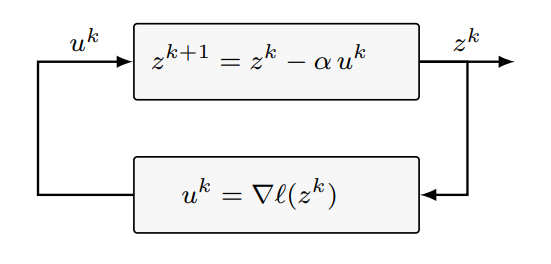
\includegraphics[width=0.45\textwidth]{figures/gradmthd}
\end{figure}


This is known as the \emph{Lur'e problem}

\section{steady-state analysis of the gradient method}
Assume that the state $z^k$ converges to some value $z_{eq}$. Then, such an equilibrium must satisfy: 
\begin{align*}
    z_{eq} = z_{eq}-\alpha\nabla\ell(z_{eq}) & \implies && z_{eq}:\nabla\ell(z_eq)\\ 
     & \implies && z_{eq} = z^*
\end{align*}
Consider the change of coordinates $z^k\to \tilde{z}^k-z_{eq}=z^k-z^*$. Then, the error dynamics is  
\begin{align*}
    \tilde{z}^{k+1} &= \tilde{z}^k-\alpha u^k \\
     u^k &= \nabla\ell(\tilde{z}^k+z^*)-\nabla\ell(z^*)
\end{align*}
where $u^k$ and $\tilde{z}^k$ satisfy, in light of the assumption on $\ell$, the following inequality\footnote{For all $z_A,z_B$ it holds that $$
    \left(\nabla\ell(z_A)-\nabla\ell(z_B)\right)^\top (z_A-z_B)\geq \displaystyle\frac{\mu L }{\mu + L} \|z_A - z_B\|^2 + \displaystyle\frac{1}{\mu + L}\|\nabla\ell(z_A)-\nabla\ell(z_B)\|^2
$$ } 
\[
    -(u^k)^T\tilde{z}^k \leq -\gamma_1\|\tilde{z}^k\|^2-\gamma_2\|u^k\|^2
\]
Consider a Lyapunov function $V:\R^d\to \R_{\geq0}$ given by $V(\tilde{z})=\|\tilde{z}\|^2$. Then 
\begin{align*}
    V(\tilde{z}^{k+1})-V(\tilde{z}^k) &= \|\tilde{z}^{k+1}\|^2-\|\tilde{z}^k\|^2\\
    &= \|\tilde{z}^k\|^2 - 2\alpha(u^k)^\top\tilde{z}^k+\alpha^2\|u^k\|^2-\|\tilde{z}^k\|^2\\ 
    &\leq -2\alpha\gamma_1 \|\tilde{z}^k\|^2 + \alpha(\alpha-2\gamma_2)\|u^k\|^2
\end{align*}
For a small enough stepsize $\alpha$ (i.e., $\alpha\leq 2\gamma_2$), we can write 
\begin{align*}
    V(\tilde{z}^{k+1})-V(\tilde{z}^k)<-2\alpha\gamma_1\|\tilde{z}^k\|^2 \quad \implies \quad \|\tilde{z}^{k+1}\|^2 & \leq (1-2\alpha\gamma_1) \|\tilde{z}^k\|^2\\ 
    & \leq (1-2\alpha\gamma_1)^k\|\tilde{z}^0\|^2
\end{align*}
Therefore $\{\tilde{z}^k\}_{k\in\\N}$ goes exponentially/geometrically fast to zero
\subsection{Gradient method for quadratic programs}
Consider a quadratic program 
\[
    \min_z \displaystyle\frac{1}{2} z^\top Q z + r^\top z
\]
With $Q=Q^\top>0$
The gradient method is an affine linear system 
\begin{align*}
    z^{k+1} &= z^k -\alpha(Qz^k+r) \qquad z^k \text{ given}\\ 
    &= (I-\alpha Q) z^k - \alpha r
\end{align*}
For a sufficiently small $\alpha$, the state matrix $(I-\alpha Q)$ is Schur. Hence, the state trajectory is \footnote{The geometric series $\sum_{i=0}^{\infty}\rho^i$ is equal to $(1-\rho)^{-1}$ for all $\rho<1$} 
\[
    z^k = (I-\alpha Q)^kz^0 - \alpha \displaystyle\sum_{i=0}^{k-1}(I-\alpha Q)^ir \to^{k\to\infty} -\alpha\left(\displaystyle\sum_{i=0}^{\infty}(I-^\alpha Q)^i\right)r = -Q^{-1}r
\]
\subsection{Gradient flow}
Let us swap the roles of the plant (the static nonlinearity) and the controller (the integrator)
\begin{figure}[h]
    \center
    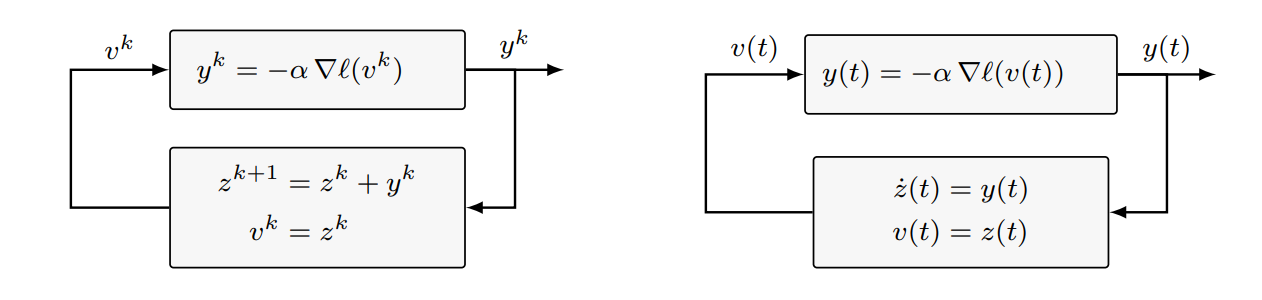
\includegraphics[width=0.95\textwidth]{figures/gradflow3}
\end{figure}
We obtain the so-called gradient flow (continuous-time dynamics)
\[
    \dot{z}(t) = -\nabla \ell(z(t)) \qquad z(0) = z_0
\]
\begin{remark}
    A solution to the ODE exists if the vector field is Lipschitz continuous
\end{remark}
\subsection{Nesterov accelerated gradient method}
Consider the following two-step algorithm: for all $k\in\N$
\[
    \zeta^{k+1} = \zeta^k + \alpha_1(\zeta^k-\zeta^{k+1}) - \alpha_2\nabla\ell \left(\zeta^k + \alpha_1(\zeta^k-\zeta^{k+1})\right), \quad \zeta^0, \zeta^{-1} \text{ given}
\]
for some $\alpha_1,\alpha_2>0$. It admits the state-space representation
\begin{figure}[H]
    \begin{center}
        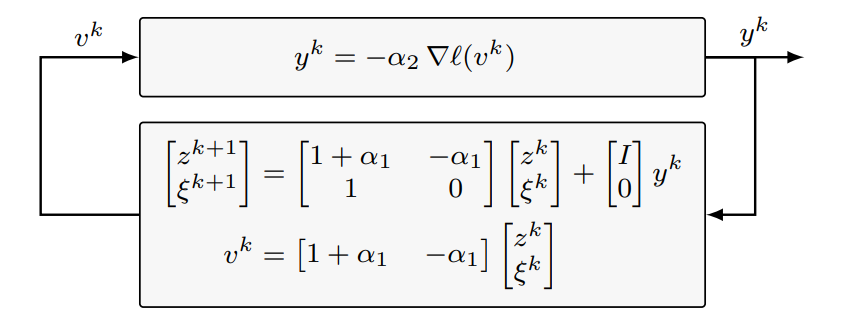
\includegraphics[width=0.45\textwidth]{figures/nesterov.png}
    \end{center}
\end{figure}

More general updates can also be considered: for all $k\in\N$
\[
    \zeta^{k+1} = \zeta^k + \alpha_1(\zeta^k-\zeta^{k+1})-\alpha_2\nabla\ell\left(\zeta^k+\alpha_3(\zeta^k-\zeta^{k-1})\right), \quad \zeta^0,\zeta^{-1} \text{ given}
\]
for some $\alpha_1, \alpha_2, \alpha_3>0$

\chapter{Parallel Optimization and Federated Learning}
\subsubsection{Cost-coupled optimization for learning}
In learning applications, we usually consider optimization problems in the form 
\[
    \min_{z\in\R^d}\displaystyle\sum_{i=1}^{N}\ell_i(z)
\]
where, for all $i=1,\dots,N$, the cost function $\ell_i:\R^d\to \R$ is local and private 
\subsubsection{(Batch) gradient method for learning}
Consider the optimization problem 
\[
    \min_z \displaystyle\sum_{i=1}^{N}\ell_i(z)
\]
The (batch) gradient method is: for each iteration $k\in\N$ 
\[
    z^{k+1} = z^k -\alpha \displaystyle\sum_{i=1}^{N}\nabla\ell_i(z^k)
\]
\begin{remark}
    computation can be expensive
\end{remark}
\section{Incremental gradient method}
Consider the optimizatio problem
\[
    \min_z \displaystyle\sum_{i=1}^{N}\ell_i(z)
\]
Idea: rather than using the whole batch gradient at each $k\in\N$, just select one single "sample" per iteration. 

The \emph{incremental gradient method} is: for each iteration $k\in\N$
\[
    z^{k+1} = z^k - \alpha\nabla\ell_{i^k}(z^k)
\]
where $i^k\in\{1,\dots,N\}$. 

Two rules for choosing index $i^k$ at iteration $k$: 
\begin{itemize}
    \item Cyclic rule: choose $i^k = 1,2,\dots,N,1,2,\dots,N,\dots$
    \item Randomized rule: draw $i^k\in\{ 1,\dots,N \}$ at random\footnote{Each $i^k$ is a realization of a discrete random variable $\mathcal{X}~\mathcal{U}\{1,N\}$ in which every one of the $N$ possible outcome values has an equal probability}, e.g according to a discrete uniform distribution
\end{itemize}
\section{Stochastic Gradient Descent}
consider the stochastic optimization problem 
\[
    \min_z \mathbb{E}_{\mathcal{W}}[\ell(z,\mathcal{W})]
\]
where $\mathbb{E}_{\mathcal{W}}[\cdot]$ denotes the expected value with respect to the random variable $\mathcal{W}$ (possibly having an uknown probability distribution $p_{\mathcal{W}}(w))$
\begin{remark}
    for all $z$, also $\ell(z,\mathcal{W})$ is a random variable, whose probability distribution depends on $p_{\mathcal{W}}$ and $\ell$. Moreover, the gradient $\nabla\ell(z,\mathcal{W})$ at each $z$ is a random quantity
\end{remark}
Assumption: There exsists an oracle that, given a realization $\bar{w}$ of $\mathcal{W}$, returns the corresponding realization of the gradient $\nabla\ell(\bar{z},\bar{w})$ at any query point $\bar{z}$

The stochastic gradient descent is: for each iteration $k\in\N$ draw a realization $w^k$ of $\mathcal{W}$ and update 
\[
    z^{k+1} = z^k -\alpha\nabla\ell(z^k,w^k)
\]
\subsection{Convergence}
\begin{proposition}[convergence with constant step-size]
    Assume: 
    \begin{itemize}
        \item $\ell$ is a $\mu$-strongly convex function with $L$-Lipschitz continuous gradient (uniformly in its second argument)
        \item $\nabla\ell(z,\mathcal{W})$ is an unbiased estimatee of $\nabla_z\mathbb{E}_{\mathcal{W}}[\ell(z,\mathcal{W})]$
        \item $\|\nabla\ell(z,\mathcal{W})\|\leq M$ almost surely\footnote{A sequence of random variables $\{\mathcal{X}_k\}_{k\in\N}$ converges almost surely to the rv $\mathcal{X}$ if $\mathbb{P}(\lim_{k\to\infty}\mathcal{X}_k=\mathcal{X})=1$} for some $M>0$
    \end{itemize}
    Let $\{z^k\}_{k\in\N}$ be a realized sequence of the SGD with stepsize $\alpha\leq 1/2 \mu$. Then 
    \[
        \|z^k-z^\star\|^2\leq (1-2\mu\alpha)^k\left(\|z^0-z^\star\|^2 - \displaystyle\frac{\alpha M^2}{2\mu}\right) + \displaystyle\frac{\alpha M^2}{2\mu}
    \]
\end{proposition} 
\emph{Analysis idea}: Use the sequence of realizations $w^0,w^1,\dots,w^k$ of $\mathcal{W}$ to approximate the original stochastic problem as 
\[
    \mathbb{E}_{\mathcal{W}}[\ell(z,\mathcal{W})] \approx \displaystyle\frac{1}{K}\displaystyle\sum_{k=1}^{L}\ell(z,w^k)
\]
\subsection{Stochastic mini-batch gradient method}
At each iteration $k\in\N$, one can use a set of realizations of $\mathcal{W}$ to statistically approximate the (random) gradient of $\ell$ at a given point $z^k$
\begin{remark}
    The set of realizations is denoted by $\mathcal{I}^k$ and is usually called minibatch
\end{remark}
For each $k\in\N$, choose $\mathcal{I}^k\subset \{\,\dots,N\}$ with $|\mathcal{I}^k| \ll N$. The stochastic minibatch gradient method is 
\[
    z^{k+1} = z^k - \alpha \displaystyle\sum_{i\in\mathcal{I}^k}\nabla \ell (z^k,w^i)
\]
\begin{remark}
    The minibatch can be chosen randomly or deterministically
\end{remark}
\begin{remark}
    This approach can also be applied to a "determinsitic" optimization problem
\end{remark}
\section{Beyond SGD: Adaptive Momentum Estimation (Adam)}
The ADAM algorithm reads as follows
\begin{itemize}
    \item Mean and Variance (first momentum and second momentum)
        \begin{align*}
            m^{k+1} & = \beta_1m^k+(1-\beta_1)\nabla\ell(z^k,w^k), &\text{for some } \beta\in(0,1)\\
            v^{k+1} & = \beta_2v^k+(1-\beta_2)[\nabla\ell(z^k,w^k)]^2, &\text{for some } \beta_2\in(0,1)
        \end{align*}
        where the square operation $[\cdot]^2$ is meant component-wise
    \item Construnct the descent direction
        \begin{align*}
            \hat{m} &= \displaystyle\frac{1}{1-\beta_1^{k+1}}m^{k+1}\\
            \hat{v} &= \displaystyle\frac{1}{1-\beta_2^{k+1}}v^{k+1}\\
            d^k &= -\displaystyle\frac{\hat{m}}{\sqrt{\hat{v}}+\epsilon}, \qquad \text{for some } \epsilon> 0
        \end{align*}
        where the division in the last equation is meant element-wise
    \item Update of the solution estimate 
        \[
            z^{k+1} = z^k + \alpha d^k
        \]
\end{itemize}

\section{Federated learning}
Consider the optimization problem 
\[
    \min_z \displaystyle\sum_{i=1}^{N}\ell(z;\mathcal{D}^i,p^i)
\]
Paradigm:
\begin{itemize}
    \item local private data $\mathcal{D}^i = ([\mathcal{D^i}]_1,[\mathcal{D^i}]_2,\dots,[\mathcal{D^i}]_d)$ and $p^i$
    \item learn common parameters $z^*\in\R^d$ (common neural network)
    \item communication with a parameter server
\end{itemize}

\section{Distributed learning}
Consider the optimization problem 
\[
    \min_z \displaystyle\sum_{i=1}^{N}\ell(z;\mathcal{D}^i,p^i)
\]
Paradigm:
\begin{itemize}
    \item local private data $\mathcal{D}^i = ([\mathcal{D^i}]_1,[\mathcal{D^i}]_2,\dots,[\mathcal{D^i}]_d)$ and $p^i$
    \item learn common parameters $z^*\in\R^d$ (common neural network)
    \item communication with neighbours only
\end{itemize}


\chapter{Leader-Follower networks: Containment}
Consider a network of $N$ agents communicating/interacting according to a fixed, undirected graph $G=(\{1,\dots,N\},E)$. Let $x_i(t)\in\R^d$ be the state of agent $i$ and for simplicity suppose $d=1$, i.e. $x_i(t)\in\R$.

\section{Definition}
Suppose that agents are divided into two groups: 
\begin{itemize}
    \item $N_f$ followers
    \item $N-N_f$ leaders
\end{itemize}
Define $x = \begin{bmatrix}
    x_f \\ x_l
\end{bmatrix}$ with $x_f\in\R^{N_f}$ the followers' state and $x_l\in\R^{N-N_f}$ the leaders' state.
Consistently, partition the Laplacian matrix as $L = \begin{bmatrix}
    L_f & L_{fl} \\ L_{FL}^\top & L_l
\end{bmatrix}$.
If leaders and followers run the same Laplacian-based distributed control law, then the Laplacian dynamics ca be written as 
\[
    \begin{bmatrix}
        \dot{x}_f(t) \\ \dot{x}_l(t) 
    \end{bmatrix} = -\begin{bmatrix}
        L_f & L_{fl} \\ L_{FL}^\top & L_l
    \end{bmatrix} \begin{bmatrix}
        x_f(t) \\ x_l(t)
    \end{bmatrix}
\]
\section{Control law}
Now, suppose that leaders and followers have different roles: 
\begin{itemize}
    \item $N_f$ followers running Laplacian dynamics
    \item $N-N_f$ leaders being stationary
\end{itemize}
The distributed control system is given by 
\begin{align*}
    & \dot{x}_i(t) = - \displaystyle\sum_{j\in\mathcal{N}_i}a_{ij} (x_i(t)-x_j(t)) && \forall i \in\{1,\dots,N_f\}\\
    & \dot{x}_i(t) = 0 && \forall i \in\{N_f+1,\dots,N\}
\end{align*}
and in compact form 
\[
    \begin{bmatrix}
        \dot{x}_f(t) \\ \dot{x}_l(t) 
    \end{bmatrix} = -\begin{bmatrix}
        L_f & L_{fl} \\ 0 & 0
    \end{bmatrix} \begin{bmatrix}
        x_f(t) \\ x_l(t)
    \end{bmatrix}
\]
The dynamics of the followers is given by 
\[
    \dot{x}_f(t) = -L_fx_f(t) - L_{fl}x_l
\]
where $x_l(t) = x_l(0)=x_l$
















\chapter{Leader Follower networks: Formation control}
\section{analogy with mass-spring systems}
Consider a platoon of $N$ masses such that each mass $i$ is connected with mass $i-1$ and $i+1$ through a spring with elastic constants respectively $a_{i-1,i} = a_{i,i-1}>0$ and $a_{i+1,i} = a_{i,i+1}>0$. Let $x_i\in \R$ be the position of mass $i$

The elastic force at mass $i$, $F_{e,i}(x)$ is given by 
\[
    F_{e,i}(x) = -a_{i,i-1}(x_i-x_{i-1})-a_{i,i+1}(x_i-x_{i+1})
\]
For each spring, we can write the associated elastic force as the negative gradient of the elastic (potential) energy, so that 
\[
    F_{e,i}(x) = -\displaystyle\frac{\partial}{\partial x_i}(\displaystyle\frac{1}{2}a_{i,i-1}\|x_i-x_{i-1}\|^2 + \displaystyle\frac{1}{2}a_{i,i+1}\|x_i-x_{i+1}\|^2)
\]
Let us suppose that each spring can be written as the parallel of two springs with elastic constants respectively $\frac{1}{2}a_{i,i-1}>0$ and $\frac{1}{2}a_{i,i+1}>0$.

Let $x_i\in\R$ be the positino of mass $i$. The elastic force at mass $i$, $F_{e,i}(x)$ is given by
\[
    F_{e,i} = -(\displaystyle\frac{1}{2}a_{i,i-1}+\displaystyle\frac{1}{2}a_{i,i-1})(x_i-x_{i-1}) -(\displaystyle\frac{1}{2}a_{i,i+1}+\displaystyle\frac{1}{2}a_{i,i+1})(x_i-x_{i+1}) 
\]
As before, we can write the elastic force as the negative gradient of the elastic (potential) energy, i.e.
\[
    F_{e,i}(x) = -\displaystyle\frac{\partial}{\partial x_i}(\displaystyle\frac{1}{2}\displaystyle\frac{a_{i,i-1}}{2}\|x_i-x_{i-1}\|^2 + \displaystyle\frac{1}{2}\displaystyle\frac{a_{i,i-1}}{2}\|x_i-x_{i-1}\|^2 + \displaystyle\frac{1}{2}\displaystyle\frac{a_{i,i+1}}{2}\|x_i-x_{i+1}\|^2 + \displaystyle\frac{1}{2}\displaystyle\frac{a_{i,i+1}}{2}\|x_i-x_{i+1}\|^2)
\]
The total elastic (potential) energy of the mass-spring system can be written as
\begin{align*}
    V(x) &= \displaystyle\sum_{i=1}^{N}\displaystyle\sum_{j\in \mathcal{N}_i} \displaystyle\frac{1}{2}\displaystyle\frac{a_{i,j}}{2}\|x_i-x_j\|^2\\ 
         &= \displaystyle\sum_{i=1}^{N}\displaystyle\sum_{j\in \mathcal{N}_i} V_{ij}(x_i,x_j)
\end{align*}
where we have defined $\mathcal{N}_i := \{ i-1, i+1 \}$ and $V_{ij}(x_i,x_j):=\displaystyle\frac{1}{2}\displaystyle\frac{a_{i,j}}{2}\|x_i-x_j\|^2$.

Thus, the elastic force at mass $i$ can be seen as the negative gradient of the energy, i.e. 
\begin{align*}
    F_{e,i}(x) &= -\displaystyle\frac{\partial}{\partial x_i}\displaystyle\sum_{j\in\mathcal{N}_i}\left(V_{ij}(x_i,x_j)+V_{ji}(x_j,x_i)\right)\\
               &=-\displaystyle\frac{\partial}{\partial x_i} V(x) 
\end{align*}
This formulation can be extended to more general systems in which masses are interconnected according to a topology described by an undirected graph $G=(\{1,\dots,N\},E)$

By adding a damping term on each mass, the system dynamics can be written as 
\begin{align*}
    \dot{x}_i &= v_i\\
    m_i\dot{v}_i &= -v_i - \displaystyle\frac{\partial}{\partial x_i}V(x) \quad \forall i \in \{ 1,\dots,N \}
\end{align*}
where we have considered the damping coeffiecient equal to one. 

If we assume that masses are small, we may written
\[
    v_i \approx - \displaystyle\frac{\partial}{\partial x_i} V(x)
\]
so that the dynamics may be approximated by the following firt order dynamics
\[
    \dot{x}_i = - \displaystyle\frac{\partial}{\partial x_i}V(x) \quad \forall i\in\{ 1,\dots,N \}
\]

Consider a network of $N$ agents communicating/interacting according to a fixed, undirected graph $G$. Let $x_i(t)\in\R^d$ be the state of agent $i$. Let agents run a Laplacian dynamics
\[
    \dot{x}_i = - \displaystyle\sum_{j\in\mathcal{N}_i}a_{ij}(x_i-x_j) \quad \forall i\in\{ 1,\dots,N \}
\]
We can rewrite it as 
\[
    \dot{x}_i(t) = - \displaystyle\sum_{j\in \mathcal{N}_i} \displaystyle\frac{\partial}{\partial x_i}\left(V_{ij}(x_i,x_j)+V_{ji}(x_j,x_i)\right) \quad \forall i \in \{ 1,\dots,N \}
\]
with $V_{ij}(x) = \displaystyle\frac{1}{2}\displaystyle\frac{a_{i,j}}{2}\|x_i-x_j\|^2$.

By recalling the definition of the total energy
\[
    V(x)=\displaystyle\sum_{i=1}^{N}\displaystyle\sum_{j\in\mathcal{N}_i}V_{ij}(x_i,x_j)
\]
the Laplacian dynamics 
\[
    \dot{x} = -Lx
\]
can be seen as a "gradient flow", i.e. 
\[
    \dot{x} = -\nabla V(x)
\]
Thus, the consensus configuration can be seen as a stationary point of $V$. This idea can be extended to general potential functions and applied to distributed control systems.

Consider a network of $N$ autonomous agents communicating/interacting according to a fixed, undirected graph. Let $x_i(t)\in\R^d$ be the state of agent $i$. Consider a global potential function defined as 
\[
    V(x)=\displaystyle\sum_{i=1}^{N}\displaystyle\sum_{j\in\mathcal{N}_i}V_{ij}(x_i,x_j)
\]
such that (local) minima of the potential correspond to desired configurations of the team. The gradient flow dynamics $\dot{x} = -\nabla V(x)$ turns out to be distributed. That is,
 \[
     \dot{x}_i(t) = \displaystyle\sum_{j\in\mathcal{N}_i}\displaystyle\frac{\partial}{\partial x_i}\left(V_{ij}(x_i,x_j)+V_{ji}(x_j,x_i)\right) \qquad \forall i \in \{ 1,\dots,N \}
 \]

 We can define a desired formation by assigning a set of distances, $d_{ij}$, between neighbouring agents $i$ and $J$ in a suitable graph 
 
 The main idea for formation control is to define a potential function matching the sparsity of $G$, $V^{\text{form}}(x) = \sum_{i=1}^{N}\sum_{j\in\mathcal{N}_i}V_{ij}^{\text{form}}(i,j)$, such that a configuration $x^{text{form}}$ satisfying 
 \[
     \|x_i^{\text{form}}-x_j^{\text{form}}\| = d_ij \qquad \forall (i,j)\in E
 \]
 is a minimum of $V$.

 In order to reach a formation with assigned distances $d_{ij}$, let us define 
 \[
     V_{ij}^{\text{form}}(x) = \displaystyle\frac{1}{8} \left(\|x_i-x_j\|^2-d_{ij}^2\right)^2
 \]
 with corresponding (global) potential function $V^{\text{form}}(x) = \displaystyle\sum_{i=1}^{N}\displaystyle\sum_{j\in\mathcal{N}_i}V_{ij}^\text{form}(x_i,x_j)$.

 The gradient flow dynamics of each agent $i$ is given by 
 \[
     \dot{x}_i = - \displaystyle\sum_{j\in\mathcal{N}_i}\displaystyle\frac{\partial}{\partial x_i} \left(V_{ij}^\text{form}(x_i,x_j)+V_{ji}(x_j,x_i)\right) \qquad \forall i \in \{1,\dots,N\}
 \]
 which reads as 
 \[
     \dot{x}_i = - \displaystyle\sum_{j\in\mathcal{N}_i} \left(\|x_i-x_j\|^2-d_{ij}^2\right)(x_i-x_j) \qquad \forall i \in \{1,\dots,N\}
 \]
This dynamics has multiple equilibrium points, including the desired formation in which the agents are at the assigned distances. In particular, the consensual solution $x_1=x_2=\dots=x_N$ is an (undesired) equilibrium.

Such a "degenerate" equilibrium can be avoided by means of additional "collision avoidance" potential functions $V_{ij}^\text{ca}(x_i,x_j)$ such that 
\[
    \lim_{\|x_i-x_j\|\to 0} V_{ij}^\text{ca}(x_i,x_j)=+\infty
\]
A possible solution is a barrier function given 
\[
    V_{ij}^\text{ca} = -\log(x_i-x_j)
\]
Similarly, barrier potential functions $V^\text{obs}(x_i)$, depending only on the state of agent $x_i$, can be used to avoid obstacles. 

The formation control dynamics becomes 
\[
    \dot{x}_i = - \displaystyle\frac{\partial V^\text{form}}{\partial x_i} - \displaystyle\frac{\partial V^\text{ca}(x)}{\delta x_i} - \nabla V^\text{obs}(x) \qquad \forall i\in\{1,\dots,N\}
\]

\chapter{Distributed Cost-Coupled Optimization}
Scenario: Network of $N$ agents communicating according to a digraph $G=(\{1,\dots,N\}E)$
\\Goal: define a distributed algorithm able to solve an optimization problem
\section{Cost-Coupled Optimization Set-up}
Consider the optimization problem 
\[
    \min_{z_in Z} \displaystyle\sum_{i=1}^{N}\ell_i(z)
\]
with $z\in\R^d$ 
\begin{itemize}
    \item $N$ agents communicate over graph $G$
    \item agent $i$ konws $\ell_i$ and $Z$ only 
    \item $z_i^k$ solution estimate of $i$
\end{itemize}
\section{Distributed Gradient Algorithm}
The centralized gradient algorithm reads 
\[
    z^{k+1} = z^k - \alpha^k \displaystyle\sum_{h=1}^{N} \nabla \ell_h(z^k)
\]
\begin{itemize}
    \item One single estimate $z^k\in\R^d$ initialized at some $z^0$ 
    \item $d^k = -\displaystyle\sum_{h=1}^{N}\nabla \ell_h(z^k)$
    \item $\displaystyle\sum_{h=1}^{N}\nabla \ell_h(z^k)$ not available to each agent
\end{itemize}
The distributed gradient algorithm reads
\begin{align*}
    v_i^{k+1} &= \displaystyle\sum_{j\in\mathcal{N_i}}a_{ij} z_j^k \\
    z_i^{k+1} &= v_i^{k+1} - \alpha^k \nabla\ell_i(v_i^{k+1})
\end{align*} 
with $z_i^0\in\R^d$

\section{Assumptions}
\begin{itemize}
    \item Assumption 1. Let $a_{ij},\ i,j \in \{1,\dots,N\}$ be nonnegative entries of a weighted adjacency matrix $A$ associated to the undirected and connected graph $G$, with $a_{ij}>0$ and $A$ doubly stochastic.
    \item Assumption 2. The step-size sequence $\{\alpha^k\}_{k\in\N}$ satisfies the conditions
        \[
            \alpha^k \geq 0, \qquad \displaystyle\sum_{k=0}^{\infty}\alpha^k = \infty, \qquad \displaystyle\sum_{k=0}^{\infty} (\alpha^k)^2 < \infty
        \]
    \item Assumption 3a. Let the following conditions hold 
        \begin{itemize}
            \item each $\ell_i:\R^d\to\R$ is convex and has bounded gradients, i.e., there exists a scalar $C_i>0$ such that $\|\nabla \ell_i(z)\|\leq C_i$ at any $z\in\R^d$
            \item the optimization problem has at least one optimal solution, i.e. the optimal solution set $Z^\star = \{z\in\R^d|\ell(z)=\ell^\star\}$ is nonempty, where $\ell^\star$ denotes the optimal value of the problem
        \end{itemize}
\end{itemize}
\begin{theorem}[]
    Let assumptions 1,2 and 3a hold true. Then, the sequences of local solution estimates $\{z_i^k\}_{k\in\N}, i=1,\dots,N$, generated by the Distributed Gradient Algorithm, asymptotically converge to a common solution $z^\star$ of the problem, i.e. for all $i=\,\dots,N$ it holds 
    \[
        \lim_{k\to\infty} \|z_i^k-z^\star\| = 0
    \]
    for some $z^\star$ in the optimal solution set $Z^\star$
\end{theorem}

\section{Distributed Projected Subgradient Algorithm}
The previous result can be extended to nonsmooth convex functions $\ell_i$ and $z$ constrained to a closed, convex set $Z\subseteq \R^d$ by implementing the following distributed step
\begin{align*}
    v_i^{k+1} &= \displaystyle\sum_{j\in\mathcal{N_i}}a_{ij} z_j^k \\
    z_i^{k+1} &= P_Z\left(v_i^{k+1} - \alpha^k \tilde{\nabla}\ell_i(v_i^{k+1})\right)
\end{align*}
where $P_Z(\cdot)$ denotes the Euclidean projection onto $Z$ while $\tilde\nabla\ell_i$ denotes a subgradient of $\ell_i$

Convergence to an optimal solution can be achieved by substituting Assumption 3a with 
\\Assumption 3b. Assume $Z\subseteq \R^d$ be a closed and bounded set. Let the following conditions hold 
\begin{itemize}
    \item each $\ell_i:Z\to\R$ is convex and has bounded subgradients, i.e. there exists a scalar $C_i>0$ such that $\|\tilde\nabla\ell_i(z)\|\leq C_i$ for any subgradient $\tilde\nabla\ell_i(z)$ of $\ell_i$ at any $z\in\R^d$
        \item the optimization problem has at least one optimal solution
\end{itemize}

\section{Improving the Distributed Gradient Algorithm}
recall the Distributed Gradient Algorithm 
\[
    z_i^{k+1} = \displaystyle\sum_{j\in\mathcal{N}_i}a_{ij}z_j^k + \alpha d_i^k
\]
We need to replace $d_i^k = -\nabla \ell_i(z_i^k)$ with a better descent direction. The idea is to use a local descent direction $d_i^k$ that aims at reconstructing the correct gradient
\[
    d_i^k \xrightarrow[\ k\to\infty\ ]-\displaystyle\frac{1}{N} \displaystyle\sum_{h=1}^{N}\nabla\ell_h(z_h^k)
\]

\subsection{Dynamic Average Consensus}
\begin{itemize}
    \item $N$ agents measure only a local, time-varying signal $r_i^k:\N\to\R$, for all $i=1,\dots,N$
    \item Each agent $i$ wants to estimate/track the average signal
        \[
            \bar{r}^k = \displaystyle\frac{1}{N} \displaystyle\sum_{i=1}^{N}r_i^k
        \]
\end{itemize}
Each agent $i$ maintains and updates a local estimate $s_i^k$ so that $\lim_{k\to\infty}\|s_i^k-\bar{r}^k\|=0$. A distributed algorithm based on a (perturbed) consensus is the following 
\[
    s_i^{k+1} = \displaystyle\sum_{j\in\mathcal{N}_i} a{ij} s_j^k + \left(r_i^{k+1}-r_i^k\right)
\]
with $s_i^0 = r_{i,0}$, where the first term represents a consensus term, and the second is a local innovation
\subsubsection{Convergence}
Let the first-order differences be relatively bounded, i.e. 
\[
    \|r_i^{k+1}-r_i^k\| \leq C_1
\]
for some $C_1>0$. Then, the local sequence generated by the dynamic average consensus satisfies 
\[
    \lim_{k\to\infty} \|s_i^k - \bar{r}^k\|\leq C_2
\]
for some $C_2>0$ and for all $i=1,\dots,N$
\begin{remark}
    The local states achieve a nonzero steady-state error, which is uniformly upper bounded
\end{remark}
\begin{remark}
    If $\|r_i^{k+1}-r_i^k\|\to0$, then the steady-state error is zero, i.e. perfect tracking is achieved
\end{remark}

\section{The Gradient Tracking Algorithm}
The strategy is to use the previous signal tracking mechanism to reconstruct the gradient of $\displaystyle\sum_{i=1}^{N}\ell_i$. The local signal is 
\[
    r_i^k = \nabla \ell_i(z_i^k)
\]
The local estimate $s_i^k$ is updated as
\[
    s_i^{k+1} = \displaystyle\sum_{j\in\mathcal{N}_i} a_{ij}s_j^k + \left(\nabla\ell_i(z_i^{k+1})-\nabla\ell_i(z_i^k)\right), \qquad s_i^0 = \nabla\ell_i(z_i^0)
\]
and use its opposite as local descent direction $d_i^k = -s_i^k$
\[
    d_i^k \xrightarrow[\ k\to\infty\ ]-\displaystyle\frac{1}{N} \displaystyle\sum_{h=1}^{N}\nabla\ell_h(z_h^k)
\]
\begin{remark}
    If each $\nabla_ell_i(z_i^k)$ converges to a constant value then perfect tracking is achieved
\end{remark}
\begin{remark}
    The convergence of $\nabla\ell_i(z_i^k)$ is intetwined with the convergence of $z_i^k$, e.g. to $z^\star$
\end{remark}
The Gradient Tracking Algorithm is 
\begin{align*}
    z_i^{k+1} &= \displaystyle\sum_{j\in\mathcal{N}_i} a_{ij}z_j^k - \alpha s_i^k && z_i^0\in\R\\
    s_i^{k+1} &= \displaystyle\sum_{j\in\mathcal{N}_i} a_{ij}s_j^k + \nabla\ell_i(z_i^{k+1}) - \nabla\ell_i(z_i^k) &&s_i^0=\nabla\ell_i(z_i^0)
\end{align*}

\subsection{Assumptions}
\begin{itemize}
    \item Assumption 1. Let $a_{ij},\ i,j\in\{1,\dots,N\}$ be non-negative entries of a weighted adjacency matrix $A$ associated to the undirected graph $G$, with $a_{ii}>0$ and $A$ doubly stochastic.
    \item Assumption 2. For all $i\in\{1,\dots,N\}$ each cost function $\ell_i:\R^d\to\R$ satisfies the following conditions
        \begin{itemize}
            \item it is strongly convex with coefficient $\mu>0$
            \item it has Lipschitz continuous gradient with constant $L>0$
        \end{itemize}
\end{itemize}
\begin{remark}
    Strong convexity implies uniqueness of the optimal solution $z^\star = \arg\min_x \displaystyle\sum_{i=1}^{N} \ell_i(z)$
\end{remark}
\subsection{Convergence Result}
\begin{theorem}[]
    Let assumptions 1 and 2 hold true. Then, there exists $\alpha^\star>0$ such that for all $\alpha\in(0,\alpha^\star)$ the sequences of local solution estimates $\{z_i^k\}_{k\in\N}$, $i=1,\dots,N$ generated by the Gradient Tracking algorithm asymptotically converge to a (consensual) solution $z^\star$ of the problem, i.e. for all $i=1,\dots,N$ it holds
    \[
        \lim_{k\to\infty} \|z_i^k-z^\star\| = 0
    \]
    Moreover, the convergence rate is linear/the stability is exponential, i.e., for all $i=1,\dots,N$ there exists $\rho\in(0,1)$ such that 
    \[
        \|z_i^k-z^\star\| \leq \rho \|z_i^{k-1}-z^\star\| \leq \rho^k \|z_i^0-z^\star\|
    \]
    for all $k\in\N$
\end{theorem}
























\chapter{Distributed Aggregative Optimization}
Consider $N$ robots in the plane that want to optimize their positions $z_i\in\R^2$, for all $i=1,\dots,N$ to perform multi-robot surveillance. Let:
\begin{itemize}
    \item $r_0\in\R^2$ be a target to protect 
    \item $r_i\in\R^2$ be the intruder associated to robot $i$ 
    \item $\sigma(z) = \displaystyle\frac{1}{N}\displaystyle\sum_{i=1}^{N}z_i$ is the barycenter of the robots 
    \item Local cost function of robot $i$ 
        \[
            \ell_i(z_i,\sigma(z)) = \gamma_i\|z_i-r_i\|^2 + \|\sigma(z)-r_0\|^2
        \]
\end{itemize}
with $z\in\R^{2N}$ the stack of $z_1,\dots,z_N$ and $\gamma_i>0$ being a tradeoff parameter.
\section{Aggregative optimization}
Let us consider aggregative optimization problems in the form 
\[
    \min_{z_1,\dots,z_N} \displaystyle\sum_{i=1}^{N} \ell_i(z_i,\sigma(z))
\]
where the aggregative variable $\sigma(z)$ is defined as 
\[
    \sigma(z) = \displaystyle\frac{1}{N}\displaystyle\sum_{i=1}^{N} \phi_i(z_i)
\]
where 
\begin{itemize}
    \item $z=(z_1,\dots,z_N)$, with each $z_i\in\R^{n_i}$, for all $i=1,\dots,N$
    \item $\ell_i:\R^{n_i}\times\R^d\to\R$ and $\phi_i\R^{n_i}\to\R^d$, for all $i=1,\dots,N$
\end{itemize}
For scalar states, $z_i\in\R$, the \emph{centralized gradient} method at iteration $k$ reads as 
\[
    z_i^{k+1} = z_i^k -\alpha \displaystyle\frac{\partial}{\partial z_i}\left. \left(\displaystyle\sum_{j=1}^{N}\ell_j(z_j,\sigma(z_1,\dots,z_N))\right)\right|_{z_1 = z_1^k,\dots,z_N = z_N^k}
\]
for all $i=1,\dots,N$ where $\alpha>0$ is the stepsize
\subsubsection{Gradient computation (scalar case)}
Since the cost function is a composite function, we need the chain rule to compute its derivative with respect to $z_i$ 
\begin{align*}
    &\displaystyle\frac{\partial}{\partial z_i}\left.\left(\displaystyle\sum_{j=1}^{N}\ell_j(z_j,\sigma(z_1,\dots,z_N))\right)\right|_{z_1 = z_1^k,\dots,z_N = z_N^k} \\
    =& \left.\displaystyle\frac{\partial}{\partial z_i} \ell_i(z_i,\sigma)\right|_{z_i=z_i^k, \sigma=\frac{1}{N}\sum_{j=1}^{N}\phi_j(z_j^k)}  \\
    &+\left. \sum_{j=1}^{N}\displaystyle\frac{\partial}{\partial\sigma}l_j(z_j,\sigma)\right|_{z_j=z_j^k, \sigma=\frac{1}{N}\sum_{j=1}^{N}\phi_j(z_j^k)}\cdot \left.\displaystyle\frac{\partial\sigma(z_1,\dots,z_N)}{\partial z_i}\right|_{z_1=z_1^k,\dots,z_N = z_N^k}
\end{align*}
Notice that $\displaystyle\frac{\partial\sigma(z_1,\dots,z_N)}{\partial z_i}=\displaystyle\frac{1}{N}\displaystyle\frac{d}{d z_i}\phi_i(z_i)$ can be computed locally

As in the scalar case, we use the chain rule to compute the gradient of the composite function. The $i$-th block of the gradient, denoted as $\left[\nabla\left(\displaystyle\sum_{j=1}^{N}\ell_j(z_j,\sigma(z_1,\dots,z_N))\right)\right]_i\in\R^{n_i}$, is given by
\begin{align*}
    &\left[\nabla\left(\displaystyle\sum_{j=1}^{N}\ell_j(z_j,\sigma(z_1,\dots,z_N))\right)\right]_i \\ 
    =& \left.\nabla_1\ell_i(z_i,\sigma)\right|_{z_j=z_j^k, \sigma=\frac{1}{N}\sum_{j=1}^{N}\phi_j(z_j^k)} \\ 
    &+ \left.\displaystyle\frac{1}{N}\nabla \phi_i(z_i)\right|_{z_i=z_i^k}\cdot \left.\displaystyle\sum_{j=1}^{N}\nabla_2 \ell_j(z_j,\sigma)\right|_{z_j=z_j^k, \sigma=\frac{1}{N}\sum_{j=1}^{N}\phi_j(z_j^k)}
\end{align*}
\section{Distributed aggregative optimization}
In a distributed contex, each agent $i$ 
\begin{itemize}
    \item knows only $\ell_i$ and $\phi_i$
        \item maintains an estimate $z_i^k$ of $z_i^\star$
        \item maintains an estimate $s_i^k$ of $\phi(z^k) = \displaystyle\frac{1}{N}\displaystyle\sum_{j=1}^{N}\phi_j(z_j^k)$
        \item maintains an estimate $v_i^k$ of $\displaystyle\sum_{j=1}^{N}\nabla_2 \ell_j(z_j^k,\sigma(z^k))$
\end{itemize}
The "tracking" idea of gradient tracking algorithm is applied to aggregative optimization
\begin{align*}
    & z_i^{k+1} = z_i^k - \alpha\left( \nabla_1\ell_i(z_i^k,s_i^k) + \nabla \phi_i(z_i^k)v_i^k \right) && z_i^0 \in\R^{n_i}\\
    & s_i^{k+1} = \displaystyle\sum_{j\in\mathcal{N}_i}a_{ij}s_j^k + \phi_i(z_i^{k+1})-\phi_i(z_i^k) && s_i^0 = \phi_i(z_i^0)\\
    & v_i^{k+1} = \displaystyle\sum_{j\in\mathcal{N}_i}a_{ij}v_j^k + \nabla_2\ell_i(z_i^{k+1},s_i^{k+1})-\nabla_2\ell_i (z_i^k,s_i^k) && v_i^0 = \nabla_2\ell_i(z_i^0,s_i^0)
\end{align*}
\begin{theorem}[aggregative tracking distributed optimization algorithm: convergence]
    Assume $G$ is a strongly connected and aperiodic digraph, and $A$ is doubly stochastic. Assume that each function $\ell_i$ is strongly convex, the gradients $\nabla_1\ell_i$ and $\nabla_2\ell_i$ are Lipschitz continuous, and $\phi_i$ is differentiable and Lipschitz continuous. 

    Then, there exists $\alpha^\star$ such that for all $\alpha\in(0,\alpha^\star)$ the sequences of local solution estimates $\{ z_1^k,\dots,z_N^k \}_{k\in\N}$ generated by the aggregative tracking distributed opitmization algorithm satisfy 
    \[
        \lim_{k\to\infty}\|z_i^k-z_i^\star\| = 0
    \]
    at a linear rate, for all $i=1,\dots,N$
\end{theorem}
\subsection{Extension to online aggregative optimization}
Consider a time-varying instance of the problem 
\begin{align*}
    \min_{z} & \displaystyle\sum_{i=1}^{N}\ell_i^k(z_i,\sigma^k(z))\\
    \text{subj. to }& z_i\in Z_i^k, \qquad \forall i=1,\dots,N
\end{align*}
where $Z_i^k\subset \R^{n_i}$ are local constraint sets.

The goal is to design an algorithm generating a sequence $\{z_i^k\}_{k\in\N}$ that "tracks" the solution $z^{k,\star}=(z_1^{k,\star},\dots,z_N^{k,\star})$ of the $k-th$ problem instance.

% Algorithm on slide 10 not required for exam
\begin{remark}
    A regret $R_K := \sum_{k=1}^{K}\sum_{i=1}^{N}\left(\ell_i^k(z_i^k,\sigma^k(z^k))-\ell_i^k(z_i^{k,\star},\sigma^k(z^{k,\star}))\right)$ can be introduced for the analysis. Under suitable assumptions, it can be proven that $R_K\leq C_1 + C_2K$ for some constants $C_1$ and $C_2$
\end{remark}


\chapter{Learning with Neural Networks}
In supervised learning we have labeled data whose generic element(sample) is composed by 
\begin{itemize}
    \item an input point $\mathcal{D}\in\R^d$, i.e. a vector $\mathcal{D} = ([\mathcal{D}]_1,\dots,[\mathcal{D}]_d)$ 
        \item a lebel $p\in\R$ associated to the input point
\end{itemize}
A dataset is usually made by $\mathcal{M}$ samples, i.e. $((\mathcal{D}^1,p^1),\dots,(\mathcal{D}^\mathcal{M},p^\mathcal{M}))$

Goal: reconstruct the uknown input-output map between inputs and labels\\
Strategy: approximate the map as a nonlinear function $\phi(\mathbb{u};\cdot):\R^d\to\R$ parametrized byh $\mathbb{u}$\\
Problem: find the best parameters $\mathbb{u}^\star$ based on data

\section{Basic element: the neuron model}
A generic neuron $h$ is a computational unit that 
\begin{itemize}
    \item has a set of weights $u_h\in\R^d$ 
    \item elaborates a vector $x\in\R^d$
    \item computes a scalar quantity 
        \[
            x_h^+ = \phi(x^\top u_h)
        \]
        with $\sigma:\R\to\R$ being the \emph{activation function}
\end{itemize}


\chapter{Multi-Robot Safety Controllers}
Consider a nonlinear system 
\[
    \dot{x}(t) = f(x(t),u(t)), \qquad x\in\R^n \quad u\in U\subset \R^m
\]
Let us define a safe (state) set 
\[
    X^s := \{ x\in\R^n | V^s(x)\geq0 \}
\]
for some sufficiently regular function $V^s:\R^n\to\R$

Goal: design a feedback control law $\kappa(x),\kappa:\R^n\to\R^m$ such that the set $X^s$ is forward invariant

\section{Control Barrier Functions}
Consider the time derivative of $V^s(x(t))$ along the system trajectories
\begin{align*}
    \displaystyle\frac{d}{dt}V^s(x(t)) &= \nabla V^s(x(t))^\top f(x(t)) + \displaystyle\sum_{h=1}^{m}\nabla V^s(x(t))^\top g_h(x(t))u_h(x(t))\\
                                       &= L_fV^s(x(t)) + L_gV^s(x(t))u(t)
\end{align*}
where $L_f$ and $L_g$ represent Lie derivatives.
We say that $V^s$ is a Control Barrier Function (CBF) if there exists a continuous, strictly increasing function $\gamma:\R\to\R$, with $\gamma(0)=0$, such that 
\[
    \sup_{u\in U}\{ L_fV^s(x) + L_gV^s(x)u + \gamma(V^s(x))\geq 0 \}
\]
for all $x\in\R^n$.

The above inequality induced by a CBF is called a \emph{control barrier certificate}.
\subsection{Admissible Control Space}
We can define the set of admissible (safe) controllers for a given state $x$ as 
\[
    U^s(x) = \left\{ u\in\R^m | L_fV^s(x) + L_gV^s(x)u + \gamma(V^s(x))\geq 0 \right\}
\]
i.e., the set of inputs satisfying the control barrier certificates. 
\begin{remark}
    It can be shown that (sufficiently regular) feedback controllers satisfying the above condition render $X^s$ forward invariant and asymptotically stable.
\end{remark}

\subsection{Safety Filters via Control Barrier Certificates}
Let $u^\text{ref}\in\R^m$ be a (possibly unsafe) reference input, e.g., obtained by a higher-level controller. The safety controller is designed to be "minimally invasive", i.e. it aims at altering the reference controller as little as possible. A safe policy $u = \kappa(x)$ can be designed as 
\begin{align*}
    \kappa(x) = \arg &\min_{u\in\R^m} \|u-u^\text{ref}(x)\|^2\\
                     &\text{subj. to } -L_fV^s(x) - L_gV^s(x)u - \gamma(V^s(x))\leq 0
\end{align*}


\section{Single-Robot Obstacle Avoidance: Single Integrator Model}
Consider a robot modeled as a single integrator, i.e. 
\[
    \dot{x} = u
\]
with $x\in\R^d$ being the state of the robot and $u\in\R^d$ the control input. The goal is to keep the robot at a safety distance $d$ from an obstacle.

Consider a CBF defined as 
\[
    V^s(x) = \| x - x_{text{obs}}\|^2 - d^2
\]
where $d$ denotes the safety distance to keep from the obstacle. The gradient wrt $x$ is given by 
\[
    \nabla V^s(x)  = 2(x-x_\text{obs})
\]
The safety, CBF-based policy can be computed as 
\begin{align*}
    \kappa_s (x) = &\arg \min_{u\in\R^d} \|u-u^\text{ref}(x)\|^2\\
    & \text{subj. to } -2(x-x_\text{obs})^\top u - \gamma(\|x-x_\text{obs}-d^2) \leq 0
\end{align*}
\begin{remark}
For a ginve, fixed $x\in\R^d$, the optimization problem above is a quadratic program    
\end{remark}
\begin{remark}
    The safety controller is meant to prevent collisions while being "minimally invasive" in the sense that it aims at altering the reference controller (coming from a higher level) as littel as possible
\end{remark}
\begin{remark}
    From a practical viewpoint the above problem requires a computation time, while the safety policy should be available in continuous time
\end{remark}


\section{Multi-Robot Collision Avoidance: Single Integrators}
Consider a team of $N$ robots modeled as single integrators, i.e.
\[
    \dot{x}_i = u_i
\]
with $x_i\in\R^d$ being the state of robot $i$ and $u_i\in\R^d$ being the control input. The goal is to keep the robots at a safety distance greater than $d$.

To keep the notation simpler, we consider a scalar robot state, and input, i.e. $x_i,u_i\in\R$.


\subsection{Control Barrier Function for Multi-Robot Collision Avoidance}
Consider a "pair-wise", local CBF defined as 
\[
    V_{i,j}^s (x_i,x_j) = \|x_i-x_j\|^2 - d^2
\]
where $d$ denotes the safety distance between robots $i$ and $j$. 

The gradient wrt $x_i$ and $x_j$ is given by 
\begin{align*}
    & \nabla_1 V_{i,j}^s(x_i,x_j) = 2(x_i-x_j)\\
    & \nabla_2 V_{i,j}^s(x_i,x_j) = 2(x_j-x_i)
\end{align*}
while the gradient wrt all the other states is zero.

Let $u\in\R^N$ denote the stack of inputs of the $N$ robots. The admissible control space for collision avoidance is obtained by considering the intersection of all the constraint sets related to a pair-wise control barrier certificates. Thus, 
\begin{gather*}
    U^s(x) \left\{ u\in\R^N | -\nabla_1V_{i,j}^s(x_i,x_j)^\top u_i - \nabla_2 V_{i,j}^s(x_i,x_j) u_j - \gamma V_{i,j}^s(x_i,x_j) \leq 0, \forall j \in \mathcal{N}_i, \forall i \in \{1,\dots,N\}\right\}
\end{gather*}
where $\mathcal{N}_i$ includes all the robots $j$ that may collide with robot $i$.
\begin{remark}
    If there are no apriori restrictions on the motion of the robots and they share the same area, we have $\mathcal{N}_i = \{1,\dots,N\}$. However, for some state configurations $\mathcal{N}_i$ may involve only a restricted number of neighbouring robots.
\end{remark}


\subsection{Centralized Safety Controller for Multi-Robot Collision Avoidance}
The safety, CBF-based policy is obtained by the following optimization problem
\begin{align*}
    \kappa(x) = \arg \min_{u\in\R^N} &\displaystyle\sum_{i=1}^{N} \|u_i-u_i^\text{ref}\|^2\\
    \text{subj. to } & -\nabla_1V_{i,j}^s(x_i,x_j)^\top u_i - \nabla_2 V_{i,j}^s(x_i,x_j) u_j - \gamma V_{i,j}^s(x_i,x_j) \leq 0\\ 
    & \|u_i\|\leq u_i^\text{max}\\
    & \forall j \in \mathcal{N}_i, \forall i \in\{1,\dots,N\}
\end{align*}
where $u_1^\text{ref},\dots,u_N^\text{ref}$ are reference inputs for each robot coming from a higher control layer, while $u_1^\text{max},\dots,u_N^\text{max}$ are input bounds for each robot.


\subsection{Decentralized Safety Controller for Multi-Robot Collision Avoidance}
In cooperative (distributed) multi-robot scenarios it is desirable not to have a central coordinator. A more constrained version of the problem can be formulated to obtain a decentralized solver. 

Safety controller for robot $i$: 
\begin{align*}
    \kappa(x) = \arg \min_{u\in\R^N} &\displaystyle\sum_{i=1}^{N} \|u_i-u_i^\text{ref}\|^2\\
    \text{subj. to } & -2\nabla_1V_{i,j}^s(x_i,x_j)^\top u_i - \frac{1}{2} \gamma V_{i,j}^s(x_i,x_j) \leq 0\\ 
    & \|u_i\|\leq u_i^\text{max}\\
    & \forall j \in \mathcal{N}_i
\end{align*}

\begin{remark}
    The decentralized safety controller requires robot i to receive information by all other robots that may incur in a collision. 
\end{remark}
\begin{remark}
    More complex models may be considered to take into account dynamics constraints
\end{remark}
\begin{remark}
    When more complex dynamics are considered together with input bounds, the (centralized or decentralized) optimization problem may become infeasible (safety cannot be guaranteed). More sophisticated approaches are required to synthetize safety barrier certificates with guaranteed feasibility. 
\end{remark}
\begin{remark}
    When the objectives of multiple robots conflict with the safety barrier certificates, robots might incur into a deadlock, i.e., a configuration that is safe but does not allow for task completion. 
\end{remark}


\chapter{Stability Analysis for Linear Averaging}
Consider $N$ agents in a network modeled as a graph $G$ with associated weighted adjacency matrix $A$

Linear averaging distributed algorithm 
\[
    x^{k+1}_i = \displaystyle\sum_{j\in\mathcal{N}_i}a_{ij}x_j^k, \quad x^0 \text{ is given } \quad i=1,\dots,N
\]
where $x_i^k\in\R$ is the state of agent $i$ at time $k$ and $a_{ij}\geq 0$ 

Each agent $i$ uses only the states of neighbours $j\in\mathcal{N}_i$, thus it is a distributed algorithm. The goal is to reach consensus. 

The linear averaging is 
\[
    \begin{bmatrix}
        x_1^{k+1} \\ \vdots \\ x_N^{k+1}
    \end{bmatrix} = \begin{bmatrix}
        a_{11} & \cdots & a_{1N} \\
        \vdots & \ddots & \vdots \\
        a_{N1} & \cdots & a_{NN} \\
    \end{bmatrix} \begin{bmatrix}
        x_1^{k} \\ \vdots \\ x_N^{k}
    \end{bmatrix}, \qquad x^0 = \begin{bmatrix}
        x_1^{0} \\ \vdots \\ x_N^{0}
    \end{bmatrix}
\]
and can be compactly written as 
\[
    x^{k+1} = Ax^k, \qquad x^0 = \begin{bmatrix}
        x_1^{0} \\ \vdots \\ x_N^{0}
    \end{bmatrix}
\]
with $x^k\in\R^n$ and the matrix $A\in\R^{N\times N}$ "compatible" with the graph $G$.
We want to study the stability properties of the equilibrium point(s) of such an autonomous system

The compact version of the linear averaging is an LTI dynamical system
\[
    x^{k+1} = A x^k \qquad x^0 \text{ given}
\]
The equilibrium points can be computed as 
\[
    x_{\text{eq}} = A x_{\text{eq}} \implies (I-A)x_{\text{eq}} = 0
\]
\begin{itemize}
    \item Is this linear system stable or unstable?
    \item Spectral properties of $A$ are crucial for the analysis
\end{itemize}
\section{Consensus result}
\begin{theorem}
    Consider the discrete-time averaging system with associated digraph $G$ and weighted adjacency matrix $A$. Assume $G$ is strongly connected and aperiodic, and $A$ is row stochastic. Then 
    \begin{enumerate}
        \item there exists a positive, left eigenvector $w\in\R^n$ such that 
            \[
                \lim_{k\to\infty} x^k = \boldsymbol{1} \displaystyle\frac{w^T x^0}{w^T \boldsymbol{1}} = \begin{bmatrix}
                    1 \\ \vdots \\ 1 
                \end{bmatrix} \displaystyle\frac{\sum_{i=1}^{N}w_ix_i^0}{\sum_{i=1}^{N}w_i}
            \]
            i.e., consensus is reached to $\displaystyle\frac{\sum_{i=1}^{N}w_ix_i^0}{\sum_{i=1}^{N}w_i}$
            \item if, additionally $A$ is doubly stochastic, then 
                \[
                    \lim_{k\to\infty} x^k = \begin{bmatrix}
                    1 \\ \vdots \\ 1 
                \end{bmatrix} \frac{\sum_{i=1}^{N}x_i^0}{N}
                \]
                i.e., \emph{average} consensus is reached
    \end{enumerate}
\end{theorem}


\section{Irreducible and primitive matrices}
A square matrix $A\in\R^{N\times N}$ is 
\begin{itemize}
    \item non-negative if all its entries are greater than or equal to zero and we write $A\geq 0$
        \item irreducible if $\sum_{k=0}^{N-1}A^k>0$

            Equivalently, there exists no permutation matrix $T$ such tha $TAT^\top$ is block triangular
        \item primitive if there exists an integer $k\in\{1,\dots,N\}$ such that $A^k$ is positive
        \item positive\footnote{Not to be confused with a \emph{positive definite} matrix, denoted as $A \succ 0$} if all its entries are greater than zero and we write $A>0$
\end{itemize}

\section{Spectral properties of square matrices}
The spectrum of a square matrix $A$, $spec(A)$, is the set of eigenvalues of $A$. The spectral radius, $\rho(A)$, is the minimum norm of the eigenvalues of $A$.
\begin{theorem}[Gershgoring Theorem]\label{gersh}
    For any (real or complex) square matrix $A$, it holds 
    \[
        spec(A)\subset \bigcup_{i=1}^N \left\{ s\in\mathbb{C} |\ |s-a_{ii}| \leq \displaystyle\sum_{j=1, j\neq i}^{N}|a_{ij}| \right\}
    \]
    That is, the union of disks in $\mathbb{C}$ centered at each diagonal entry $a_{ii}$ with radius $\sum_{j=1,j\neq i}^{N}|a_{ij}$
\end{theorem}
\begin{theorem}[]
    Let $G$ be a weighted digraph with $N\geq2$ nodes and with weighted adjacency matrix $A$. Then $A$ is irreducible iff $G$ is strongly connected
\end{theorem}
\begin{theorem}[]
    Let $G$ be a weighted digraph with $N\geq2$ nodes and with weighted adjacency matrix $A$. Then $A$ is primitive iff $G$ is strongly connected and aperiodic
\end{theorem}
\begin{theorem}[Perron-Frobenius theorem]
    Let $A\in\R^{N\times N}$ with $N\geq2$ be a non-negative matrix, then 
    \begin{enumerate}
        \item there exists a real eigenvalue $\lambda\geq |\mu|\geq0$ for all other eigenvalues $\mu\in\mathbb{C}$ of $A$
        \item the right eigenvector $v\in\R^N$ and left eigenvector $w\in\R^N$ associated to $\lambda$ can be selected non-negative 

            If, additionally $A\in\R^{N\times N}$ is irreducible, then 
        \item the eigenvalue $\lambda\in\R$ is striclty positive and simple
        \item the right eigenvector $v\in\R^N$ and left eigenvector $w\in\R^N$ associated to $\lambda$ are unique and positive, possibly up to rescaling

            If, additionally $A\in\R^{N\times N}$ is primitive, then
        \item The eigenvalue $\lambda>|\mu|$ for all other eigenvalues $\mu\in\mathbb{C}$ of $A$
    \end{enumerate}
\end{theorem}

\subsection{Spectral properties of row-stochastic matrices}
\begin{lemma}
    For a row-stochastic matrix $A\in\R^{N\times N}$
    \begin{enumerate}
        \item $\lambda = 1$ is an eigenvalue of $A$
        \item $\spec(A)$ is a subset of the unit disk
    \end{enumerate}
\end{lemma}
\begin{proof}[Proof]
    For the first statement, use $A\boldsymbol{1} = \boldsymbol{1}$. For the second statement use the Gershgoring Theorem \ref{gersh}
\end{proof}
\section{Application of the Perron-Frobenius theorem}
Let $A\in\R^{N\times N}$ be a row stochastic and primitive matrix. We already know that $\lambda=1$ is an eigenvalue of $A$ and $\lambda=1\geq |\mu|$ for all other eigenvalues $\mu$ (since they lie in the unit disk). Invoking the Perron-Frobenius Theorem, the eigenvalue $\lambda=1$ must be simple and strictly dominant, i.e. $1=\lambda>|\mu|$ for all other eigenvalues $\mu\in\spec(A)\backslash \{1\}$.

Therefore, the averaging system 
\[
    x^{k+1} = A x^k,\qquad x^0 \text{ given}
\]
is marginally stable. 
\subsection{Equilibrium manifold of linear averaging}
Let us investigate the equilibrium manifold of $x^{k+1} = Ax^k$. We have 
\begin{itemize}
    \item $x_{eq} = Ax_{eq} \implies x_eq\in\ker(I-A) = \vspan \boldsymbol{1} = \boldsymbol{1}\beta$ for some $\beta\in\R$
    \item $w^Tx^{k+1} = w^T Ax^k = w^Tx^k = w^Tx^0$ for all $k\in\N$
        \\ Hence also $w^Tx^0=w^Tx_{eq}=w^T\boldsymbol{1}\beta\implies \beta = (w^Tx^0)/(w^T\boldsymbol{1})$
    \item Thus: $x_{eq} = \boldsymbol{1} \displaystyle\frac{w^Tx^0}{w^T\boldsymbol{1}}$
\end{itemize}
\begin{remark}
    The equilibrium is not necessarily the origin and depends on the initial condition $x^0$
\end{remark}
\begin{remark}
    Wlog, we condsider a rescaled version of $w$, so that $w^T\boldsymbol{1}=1$
\end{remark}
\section{Convergence proof (I): Jordan form approach}
Being $G$ strongly connected and aperiodic, then $A$ is also primitive (other than being row stochastic). Hence, 
\begin{itemize}
    \item it has one dominant eigenvalue in $1$ associated to eigenvectors $\boldsymbol{1}\in\R^N$ (right) and $w\in\R^N$ (left)
    \item it has $N-1$ eigenvalues with norm strictly less than 1
\end{itemize}
Consider the change of coordinates 
\[
    x \longmapsto \tilde{x} = T^{-1}x
\]
with the nonsingular matrix $T\in\R^{N\times N}$ being associated to the Jordand form $T^{-1}AT$ of $A$
\[
    T^{-1} A T = \left[\begin{array}{c| c c c }
        1 & & & \\ \hline \\ & & J_2 & \\ & & & 
    \end{array}\right]
\]
with $J_2\in\R^{(N-1) \times (N-1)}$ Schur (the empty spaces are zeros)

Let matrix $T$ be arranged as 
\[
    T = \left[\begin{array}{c | c c c}
        \uparrow & \uparrow & & \uparrow\\ 
        \boldsymbol{1} & v^2 & \cdots & v^N \\
        \downarrow & \downarrow & & \downarrow
    \end{array}\right] = \left[\begin{array}{c | c}
        \boldsymbol{1} & W_L
    \end{array}\right] \quad \text{and} \quad T^{-1} = \left[\begin{array}{c c c}
        \leftarrow &  w^T   &\rightarrow \\ \hline
        \leftarrow &  {w^2}^T   &\rightarrow \\
         &  \vdots   &\\
        \leftarrow &  {w^N}^T   &\rightarrow \\
    \end{array}\right] = \left[\begin{array}{c}
        w^T \\ \hline
        W_R
    \end{array} \right]
\]
with $W_L\in\R^{N\times (N-1)}$ and $W_R\in\R^{(N-1)\times N}$

The dynamics of $x^{k+1}=Ax^k$ in the new coordinates is 
\[
    x \longmapsto \tilde{x} = T^{-1}x \quad \implies \quad \tilde{x}^{k+1} = T^{-1}AT\tilde{x}^k = \left[\begin{array}{c| c c c }
        1 & & & \\ \hline \\ & & J_2 & \\ & & & 
    \end{array}\right] \tilde{x}^k, \qquad \tilde{x}^0 = T^{-1}x^0
\]
with $J_2$ Schur

From the definition of $T^{-1}$, for all $k\in\N$ we have $\tilde{x}^k=(\tilde{x}_m^k,\tilde{x}_\perp^k)$ with 
\begin{itemize}
    \item $tilde{x}_m^k = w^T x^k\in\R$ being the weighted average of $x^k$ 
    \item $\tilde{x}_\perp^k=W_R^Tx^k\in\R^{N-1}$ being the remaining components (dispersion) 
\end{itemize}
Then 
\[
    \lim_{k\to\infty} \tilde{x}^k = \lim_{k\to\infty} \left[\begin{array}{c}
        \tilde{x}_m^k \\ \\ \tilde{x}_\perp^k
    \end{array}\right] = \lim_{k\to\infty}\left[\begin{array}{c| c c c }
        1 & & & \\ \hline \\ & & J_2 & \\ & & & 
    \end{array}\right]^k \left[\begin{array}{c}
        \tilde{x}_m^0 \\ \\ \tilde{x}_\perp^0
    \end{array}\right] = \lim_{k\to\infty} \left[\begin{array}{c}
        1^k \tilde{x}_m^0 \\ \\ J_2^k\tilde{x}_\perp^0
    \end{array}\right] = \left[\begin{array}{c}
        \tilde{x}_m^0 \\ 0 \\ \vdots \\ 0
    \end{array}\right]
\]
where, by definition, $\tilde{x}_m^0=w^Tx^0$

Therefore, in the original coordinates, it holds 
\[
    \lim_{k\to\infty} x^k = \lim_{k\to\infty} T\tilde{x}^k = \left[\begin{array}{c}
        \tilde{x}_m^0 \\ \vdots \\ \tilde{x}_m^0
    \end{array}\right] = \boldsymbol{1}w^Tx^0
\]
\subsection{The dissensus dynamics}
Consider the so-called delated matrix defined as 
\[
    A- \boldsymbol{1}w^T\in\R^{N\times N}
\]
that, differently from $A$, is Schur. In fact, the simple eigenvalue in 1 of $A$ has been "moved" to 0
\\Define the \emph{dissensus} vector in $\R^N$ as 
\[
    \delta^k := x^k- \boldsymbol{1}w^Tx^0 = (I-\boldsymbol{1}w^T)x^k
\]
for all $k\in\N$
\begin{remark}
    If the dissensus is zero, it means that consensus has been achieved
\end{remark}
The dissensus dynamics is 
\[
    \delta^{k+1} = (A-\boldsymbol{1}w^T)\delta^k, \qquad \delta^0 = (I-\boldsymbol{1}w^t)x^0
\]
\section{Convergence proof (II): Lyapunov approach}
Consider the Jordan form of the deflated matrix
\[
    J = T^{-1} (A-\boldsymbol{1}w^T)T = \left[\begin{array}{c| c c c }
        0 & & & \\ \hline \\ & & J_2 & \\ & & & 
    \end{array}\right] \implies (A-\boldsymbol{1}w^T) = TJT^{-1}
\]
with $T\in\R^{N\times N}$ nonsingular.

For all $Q_2=Q_2^T \succ 0 \in\R^{(N-1)\times(N-1)}$, there exists a matrix $P_2=P_2^T \succ 0 \in\R^{(N-1)\times(N-1)}$ and a scalar $p_1>0$ satisfying the following (discrete-time) Lyapunov equation
\[
    \left[\begin{array}{c| c c c }
        0 & & & \\ \hline \\ & & J_2 & \\ & & & 
    \end{array}\right]^T \left[\begin{array}{c| c c c }
        p_1 & & & \\ \hline \\ & & P_2 & \\ & & & 
    \end{array}\right] \left[\begin{array}{c| c c c }
        0 & & & \\ \hline \\ & & J_2 & \\ & & & 
    \end{array}\right] - \left[\begin{array}{c| c c c }
        p_1 & & & \\ \hline \\ & & P_2 & \\ & & & 
    \end{array}\right] = \left[\begin{array}{c| c c c }
        -p_1 & & & \\ \hline \\ & & -Q_2 & \\ & & & 
    \end{array}\right]
\]
Consider the congruence transformation (preserving the sign of the eigenvalues)
\[
    P \longmapsto \Pi := (T^{-1})^T \left[\begin{array}{c| c c c }
        p_1 & & & \\ \hline \\ & & P_2 & \\ & & & 
    \end{array}\right] T^{-1} \qquad \implies \quad P = T^T\Pi T
\]
and choose the Lyapunov function $V_\Pi:\R^N\to \R_{\geq0}$ 
\[
    V_\Pi(\delta) := \delta^T\Pi\delta
\]
Then its increment along trajectories satisfies
\begin{align*}
    V_\Pi(\delta^{k+1})-V_\Pi(\delta^k) &= (\delta^k)^T(A-\boldsymbol{1}w^T)^T\Pi(A-\boldsymbol{1}w^T)\delta^k-(\delta^k)^T\Pi\delta^k \\
    &= (\delta^k)^T(TJT^{-1})^T\Pi(TJT^{-1})\delta^k - (\delta^k)^T\Pi\delta^k \\ 
    &= (T^{-1}\delta^k)^T(J^TT^T\Pi TJ-T^T\Pi T)T^{-1}\delta^k \\ 
    &= (T^{-1}\delta^k)^T \left[\begin{array}{c|c}
        -p_1 & \\ \hline & -Q_2 T^{-1}\delta^k
    \end{array}\right] \\ 
    &= -\|T^{-1}\delta^k\|^2_Q < 0
\end{align*}

\section{Convergence proof (III): alternative Lyapunov approach}
Consider the so-called max-min disagreement function $V_{m-m}:\R^N\to\R_{\geq0}$
\[
    V_{m-m}(x) = \left(\max_{i\in\{1,\dots,N\}}x_i\right) - \left(\min_{i\in\{1,\dots,N\}}x_i\right)
\]
\begin{itemize}
    \item it is a non-quadratic candidate Lyapunov function
    \item Notice that $V_{m-m}(x)=0$ iff $x = \boldsymbol{1}\beta$ for some $\beta\in\R$
    \item its increment along trajectories decreases monotonically, i.e. for all $k$  
        \[
            V_{m-m}(Ax^k)<V_{m-m}(x^k)
        \]
\end{itemize}
Invoking the Lyapunov theorem, we can conclude that $x^k\xrightarrow[\ k\to\infty\ ]{} \boldsymbol{1} \beta$
\\Since we have shown that the equilibrium is $\beta=w^Tx^0$, it follows that $x^k\xrightarrow[k\to\infty]{}\boldsymbol{1}w^Tx^0$



\chapter{Gradient tracking analysis}
In the gradient tracking each agent $i$ performs 
\begin{align*}
    z_i^{k+1} &= \displaystyle\sum_{j\in\mathcal{N}_i}a_{ij}z_j^k - \alpha s_i^k && z_i^0\in\R\\
    s_i^{k+1} &= \displaystyle\sum_{j\in\mathcal{N}_i}a_{ij}s_j^k + \nabla\ell_i(z_i^{k+1})-\nabla\ell_i(z_i^k) && s_i^0 = \nabla\ell_i(z_i^0)
\end{align*}
\subsubsection{Aggregate reformulation}
Let 
\[
    z^k = \begin{bmatrix}
        z_1^k \\ \vdots \\ z_N^k
    \end{bmatrix} \qquad s^k = \begin{bmatrix}
        s_1^k \\ \vdots \\ s_N^k
    \end{bmatrix} \nabla\boldsymbol{\ell}(z^k) = \begin{bmatrix}
        \nabla\ell_1(z_1^k) \\ \vdots \\ \nabla\ell_N(z_N^k)
    \end{bmatrix}
\]
Then, the gradient tracking can be compactly written as 
\begin{align*}
    z^{k+1} &= Az^k - \alpha s^k && z^0 \in \R^n \\
    s^{k+1} &= As^k - \nabla\boldsymbol{\ell}(z^{k+1}) - \nabla\boldsymbol{\ell}(z^{k}) && s^0  = \nabla\boldsymbol{\ell}(z^{0})
\end{align*}
where $A\in\R^{N\times N}$ is the matrix collecting the weights $a_{ij}$
\begin{remark}
    It is not a causal dynamical system
\end{remark}

\section{Equilibrium manifold for the Gradient Tracking}
The equilibrium of the system $(z_{eq},s_{eq})$ must satisfy
\begin{align*}
    & z_{eq} = A z_{eq}-\alpha s_{eq} \\
    & s_{eq} = A s_{eq} + \nabla\boldsymbol{\ell}(z_{eq}) - \nabla\boldsymbol{\ell}(z_{eq})
\end{align*}
Therefore 
\begin{itemize}
    \item from the second: $s_{eq}\in\ker(I-A)=\vspan \boldsymbol{1} \implies s_{eq} =\boldsymbol{1}\beta_1$ for some $\beta_1\in\R$
    \item from the first: $(I-A)z_{eq} = -\alpha\boldsymbol{1}\beta_1$. But since $\ker(I-A)=\vspan \boldsymbol{1}$ it must be $\beta_1=0$ and  
        \begin{align*}
            &s_{eq} = 0 \\
            &z_{eq} = \boldsymbol{1} \beta_2 \text{ for some } \beta_2 \in\R
        \end{align*}
\end{itemize}
Moreover, by pre-multiplying by $\boldsymbol{1}^T$ the second state equation, for all $k\in\N$ we have
\begin{align*}
    \boldsymbol{1}^T s^{k+1} &= \boldsymbol{1}^T A s^{k} +\boldsymbol{1}^T \nabla\boldsymbol{\ell}(z^{k+1} -\boldsymbol{1}^T \nabla\boldsymbol{\ell}(z^{k})\\ 
    &= \boldsymbol{1}^T s^k+\boldsymbol{1}^T \nabla\boldsymbol{\ell}(z^{k+1}) -\boldsymbol{1}^T \nabla\boldsymbol{\ell}(z^{k}) 
\end{align*}
This implies an invariance condition 
\begin{align*}
    \boldsymbol{1}^T s^{k+1} -\boldsymbol{1}^T \nabla\boldsymbol{\ell}(z^{k+1} &=  s^{k}  -\boldsymbol{1}^T \nabla\boldsymbol{\ell}(z^{k})\\ 
    &= \boldsymbol{1}^Ts_{eq}-\boldsymbol{1}^T \nabla\boldsymbol{\ell}(z^{eq}) = 0 - \boldsymbol{1}^T\nabla\boldsymbol{\ell}(z_{eq}) = -\boldsymbol{1}^T\nabla\boldsymbol{\ell}(\boldsymbol{1}\beta_2)\\ 
    &= \boldsymbol{1}^Ts_{0}-\boldsymbol{1}^T \nabla\boldsymbol{\ell}(z^{0}) = 0
\end{align*}
Therefore it must be $\beta_2=z^\star$, so that $z_{eq} =\boldsymbol{1}z^\star$

\section{Causal coordinates for the Gradient Tracking}
Consider the nonlinear change of coordinates 
\[
    \begin{bmatrix}
        z^k \\ s^k
    \end{bmatrix} \mapsto \begin{bmatrix}
        z^k \\ \xi^k
    \end{bmatrix} = \begin{bmatrix}
        z^k \\ \alpha(\nabla\boldsymbol{\ell}(z^k)-s^k)
    \end{bmatrix}
\]
\begin{remark}
    The inverse transformation is $s^k = -\frac{1}{\alpha}\xi^k + \nabla \boldsymbol{\ell}(z^k)$
\end{remark}
The GT dynamics in the new coordinates is 
\begin{align*}
    z^{k+1} &= Az^k + \xi^k - \alpha\nabla\boldsymbol{\ell}(z^k) && z^0\in\R^N\\
    \xi^{k+1} &= A\xi^k - \alpha(A_I)\nabla\boldsymbol{\ell}(z^k) && \xi^0 = 0
\end{align*}
\begin{remark}
    This is a causal system
\end{remark}

\subsection{Block diagram of the Gradient Tracking Algorithm}
\begin{figure}[H]
    \begin{center}
        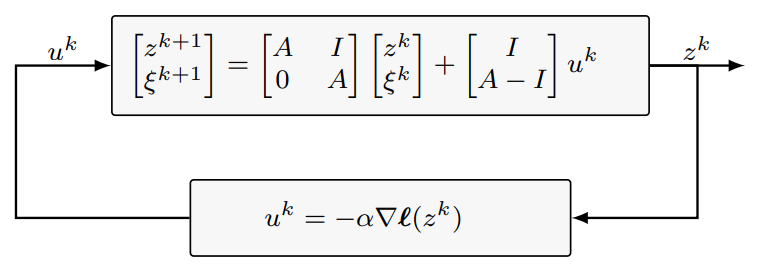
\includegraphics[width=0.95\textwidth]{figures/gradtrack}
    \end{center}
\end{figure}
\begin{itemize}
    \item The upper part is a linear dynamical system with states $(z,\xi)$ and input $u$ (and output $y=z$)
    \item The state matrix $\begin{bmatrix}
            A & I \\ 0 & A
    \end{bmatrix}$ is Schur except for the semi-simple eigenvalue in $1$ (geom. mult. 2)
    \item The step-size $\alpha>0$ plays the role of a gain
    \item the lower part is a static nonlinearity (as in the gradient method)
\end{itemize}

\section{Local perspective of the causal GT}
From a local perspective, each agent $i$ performs 
\begin{align*}
    z^{k+1}_i &= \displaystyle\sum_{j\in\mathcal{N}_i}a_{ij}z_j^k + \xi_i^k - \alpha\nabla\ell_i(z_i^k) && z_i^0\in\R^N\\
    \xi_i^{k+1} &= \displaystyle\sum_{j\in\mathcal{N}_i}a_{ij}\xi_j^k - \alpha\left(\displaystyle\sum_{j\in\mathcal{N}_i}a_{ij}\nabla\ell_j(z_j^k) - \nabla\ell_i(z_i^k)\right) && \xi_i^0 = 0
\end{align*}
\begin{remark}
    more communication is needed in these coordinates
\end{remark}
Since each cost function $\ell_i$ is strongly convex (with parameter $\mu>0$) with Lipschitz continuous gradient (with parameter $L>0$) then for all $z_A, z_B\in\R^N$ it holds 
\begin{align*}
    (\nabla\boldsymbol{\ell}(z_A)-\nabla\boldsymbol{\ell}(z_B))^T(z_A-z_B) &= \displaystyle\sum_{i=1}^{N} (\nabla\ell_i(z_{i,A})-\nabla\ell_i(z_{i,B}))^T(z_{i,A}-a_{i,B})\\ 
    &\geq \displaystyle\frac{\mu L}{L + \mu}\|z_A-z_B\|^2 + \displaystyle\frac{1}{L + \mu}\|\nabla\boldsymbol{\ell}(z_A)-\nabla\boldsymbol{\ell}(z_B)\|^2
\end{align*}

\section{Error coordinates for the Gradient Tracking}
Consider the error coordinates 
\[
    \begin{bmatrix}
        z^k \\ \xi^k
    \end{bmatrix} \mapsto \begin{bmatrix}
        \tilde{z}^k \\ \tilde{\xi}^k
    \end{bmatrix} = \begin{bmatrix}
        z^k - \fatone \\ \xi^k - \alpha\nabla\fatl(\fatone z^\star)
    \end{bmatrix}
\]
The dynamics in the new coordinates is 
\begin{align*}
    \tilde{z}^{k+1} &= A \tilde{z}^k + \tilde{\xi}^k - \alpha \left(\nabla\fatl(z^k)-\nabla\fatl(\fatone z^\star)\right) && \tilde{z}^0 \text{ given}\\
    \tilde{\xi}^{k+1} &= A \tilde{\xi}^k - \alpha (A_I)(\nabla\fatl(z^k)-\nabla\fatl(\fatone z^\star)) && \tilde{\xi}^0 \text{ given}
\end{align*}
that can be written as 
\[
    \begin{bmatrix}
        \tilde{z}^{k+1} \\ \tilde{\xi}^{k+1}
    \end{bmatrix} = \begin{bmatrix}
        A & I \\ 0 & A
    \end{bmatrix} \begin{bmatrix}
        \tilde{z}^{k} \\ \tilde{\xi}^{k}
    \end{bmatrix} - \alpha \begin{bmatrix}
        I \\ A_I
    \end{bmatrix} (\nabla\fatl(\tilde{z}^k+\fatone z^\star)-\nabla\fatl(\fatone z^\star))
\]
\begin{remark}
    The equilibrium has been shifted to the origin $(\tilde{z},\tilde{\xi}) = (0,0)$
\end{remark}

\subsection{Block diagram of the Gradient Tracking in error coordinates}
\begin{figure}[h]
    \begin{center}
        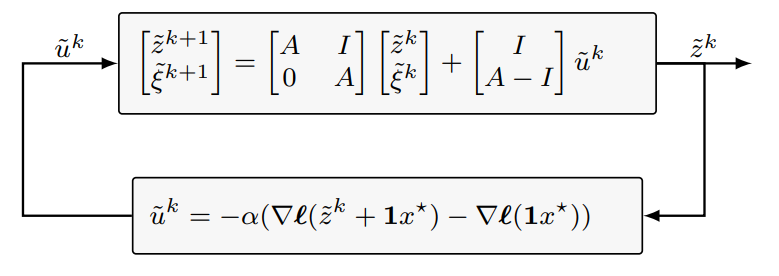
\includegraphics[width=0.95\textwidth]{figures/trackerr}
    \end{center}
\end{figure}
\begin{itemize}
    \item The origin $(\tilde{z},\tilde{\xi}) = (0,0)$ is the equilibrium
    \item The feedback action $\tilde{u}^k$ is a static map whose characterization depends on the regularity properties of the cost function, i.e. $(\mu,L)$, and is given by
        \[
            (\nabla\boldsymbol{\ell}(\tilde{z}^k+\fatone z^\star)-\nabla\boldsymbol{\ell}(\fatone z^\star))^T \tilde{z}^k \geq \displaystyle\frac{\mu L}{L + \mu}\|\tilde{z}^k\|^2 + \displaystyle\frac{1}{L + \mu}\|\nabla\boldsymbol{\ell}(\tilde{z}^k+\fatone z^\star)-\nabla\boldsymbol{\ell}(\fatone z^\star)\|^2
        \]
        \item The feedback must be a stabilizing action for the closed-loop system
\end{itemize}

\section{Analysis sketch}
Let us focus on the upper (open-loop) linear system
\[
    \begin{bmatrix}
        \tilde{z}^{k+1} \\ \tilde{\xi}^{k+1}
    \end{bmatrix} = \begin{bmatrix}
        A & I \\ 0 & A
    \end{bmatrix} \begin{bmatrix}
        \tilde{z}^{k} \\ \tilde{\xi}^{k}
    \end{bmatrix} + \begin{bmatrix}
        I \\ A_I
    \end{bmatrix} \tilde{u}^k
\]
Let us consider a change of coordinates (with $T_z = \left[\begin{array}{lr}
    \fatone & W
\end{array}\right]$ and $T_\xi = \left[\begin{array}{cc}
    W & \fatone 
\end{array}\right])$, orthonormal) given by 
\[
    \begin{bmatrix}
        \tilde{z}^k \\ \tilde{\xi}^k
    \end{bmatrix} \mapsto \begin{bmatrix}
        \begin{bmatrix}
            \tilde{z}^k_m \\ \tilde{z}^k_\perp
        \end{bmatrix} \\ \begin{bmatrix}
            \tilde{\xi}^k_\perp \\ \tilde{\xi}^k_m
        \end{bmatrix}
    \end{bmatrix} = \left[\begin{array}{c|c}
        T_z^T & \\ \hline & T_\xi^T
    \end{array}\right] \begin{bmatrix}
        \tilde{z}^k \\ \tilde{\xi}^k
    \end{bmatrix}
\]
The dynamics in the new coordinates reads 
\[
    \begin{bmatrix}
        \tilde{z}^{k+1}_m \\ \tilde{z}^{k+1}_\perp \\ \tilde{\xi}^{k+1}_\perp \\ \tilde{\xi}^{k+1}_m
    \end{bmatrix} = \begin{bmatrix}
        1 & 0 & 0 & 1 \\ 
        0 & J_2 & I_{N-1} & 0\\
        0 & 0 & J_2 & 0 \\
        0 & 0 & 0 & 1 \\
    \end{bmatrix} \begin{bmatrix}
        \tilde{z}^{k}_m \\ \tilde{z}^{k}_\perp \\ \tilde{\xi}^{k}_\perp \\ \tilde{\xi}^{k}_m
    \end{bmatrix} + \begin{bmatrix}
        \fatone^T \\ W^T \\ W^T(A-I) \\ 0
    \end{bmatrix} \tilde{u}^k
\]
where $J_2:= W^TAW$ is Schur

It can be shown that 
\begin{enumerate}
    \item the matrix $F_{22} = \begin{bmatrix}
            J_2 & I_{N-1} \\ 0 & J_2
    \end{bmatrix}$ is Schur
\item $\xi_i^0 = 0$ for all $i$ implies that $\tilde{x}^0_m=0$
\end{enumerate}
Therefore the evolution of $\tilde{x}_m^k$ can be ignored to obtain a "reduced" system
\[
    \begin{bmatrix}
         \tilde{z}^{k+1}_m \\ \begin{bmatrix}
             \tilde{z}^{k+1}_\perp \\ \tilde{\xi}^{k+1}_\perp 
         \end{bmatrix}
    \end{bmatrix} = \begin{bmatrix}
        1 & 0 \\ 0 & F_{22}
    \end{bmatrix} \begin{bmatrix}
         \tilde{z}^{k}_m \\ \begin{bmatrix}
             \tilde{z}^{k}_\perp \\ \tilde{\xi}^{k}_\perp 
         \end{bmatrix}
    \end{bmatrix} + \begin{bmatrix}
        \fatone^T \\ G_2
    \end{bmatrix} \tilde{u}^k
\]
with $G_2 = \begin{bmatrix}
    W^T \\ W^T(A-I)
\end{bmatrix}$, where $\tilde{u}^k = -\alpha(\nabla\fatl(\fatone \tilde{z}^k_m + W \tilde{z}^k_\perp + \fatone z^\star)-\nabla\fatl(\fatone z^\star))$ (coupling the dynamics)

Consider the quadratic Lyapunov function
\[
    \mathcal{V}(\tilde{z}^k_m,\tilde{z}^k_\perp,\tilde{\xi}^k_\perp) = \begin{bmatrix}
         \tilde{z}^{k}_m \\ \begin{bmatrix}
             \tilde{z}^{k}_\perp \\ \tilde{\xi}^{k}_\perp 
         \end{bmatrix}
    \end{bmatrix}^T \begin{bmatrix}
        1 & 0 \\ 0 & P_2
    \end{bmatrix} \begin{bmatrix}
         \tilde{z}^{k}_m \\ \begin{bmatrix}
             \tilde{z}^{k}_\perp \\ \tilde{\xi}^{k}_\perp 
         \end{bmatrix}
    \end{bmatrix}
\]
with $P_2 = P_2^T \succ 0$ designed on the matrix $F_{22}$ (i.e., via $F_{22}^TP_2F_{22}-P_2 \prec 0$)

There exists $\alpha^\star >0$ such that for all $\alpha\in(0,\alpha^\star)$ it holds
\begin{align*}
    \mathcal{V}(\tilde{z}^{k+1}_m,\tilde{z}^{k+1}_\perp,\tilde{\xi}^{k+1}_\perp) - \mathcal{V}(\tilde{z}^k_m,\tilde{z}^k_\perp,\tilde{\xi}^k_\perp) &= \begin{bmatrix}
        \tilde{z}^{k}_m \\ \tilde{z}^{k}_\perp \\ \tilde{\xi}^{k}_\perp 
    \end{bmatrix}^T (F^TPF-P) \begin{bmatrix}
        \tilde{z}^{k}_m \\ \tilde{z}^{k}_\perp \\ \tilde{\xi}^{k}_\perp 
    \end{bmatrix} + 2 \begin{bmatrix}
        \tilde{z}^{k}_m \\ \tilde{z}^{k}_\perp \\ \tilde{\xi}^{k}_\perp 
    \end{bmatrix}^T F^TPG\tilde{u}^k + (\tilde{u}^k)^T G^T PG\tilde{u}^k \\
    &\leq -q_1\|\tilde{z}_m^k\|^2 - q_2 \|\tilde{z}^k_\perp\|^2 -q_3 \|\tilde{\xi}^k_\perp\|^2
\end{align*}
for some $q_1,q_2,q_3>0$ (depending on $\alpha$)

It follows that the origin is exponentially stable, which translates in the sought linear convergence of the solution estimates generated by the Gradient Tracking

\section{Gradient Tracking: extensions}
Gradient Tracking can be extended to handle 
\begin{itemize}
    \item Nonconvex cost functions
    \item Convex constraitns on the optimization variable
    \item Time-varying and directed communication networks (packet losses)
    \item Block-wise updates and communication
    \item Stochastic optimization problems
    \item Heavy-ball, Nesterov, Adam-like implementations
\end{itemize}

\section{System theoretical approach to distributed optimization}
\begin{itemize}
    \item Gradient tracking can be shown to implement a \emph{distributed integral action}
        \item The approach can be generalized to derive more general controllers and/or algorithms
\end{itemize}
For instance, consider the following algorithm
\begin{align*}
    z^{k+1} = Az^k - (I-A)\xi^k - \alpha\nabla\fatl(z^k) && z^0 \in\R^N\\
    \xi^{k+1} = \xi^k + (I-A)z^k && \xi^0 \in\R^N\\
\end{align*}
\begin{remark}
    THe dynamics of the controller state $\xi^k$ is a pure discrete-time integrator trying to compensate for the consensus error $(I-A)z^k$
\end{remark}









\chapter{Constraint-coupled Distributed Optimization}
Constraint-coupled optimization problem 
\begin{align*}
    \min_{z_1,\dots,z_N} & \displaystyle\sum_{i=1}^{N}\ell_i(z_i)\\
    \text{subj. to } & z_i\in Z_i \subset \R^{n_i}  \qquad  i=1,\dots,N \\
                     & \displaystyle\sum_{i=1}^{N}g_{ij}(z_i)\leq 0 \qquad j=1,\dots,r
\end{align*}
with $\ell_i:\R^{n_i}\to \R$ convex, $g_{ij}:\R^{n_i}\to\R$ convex and $Z_i\subset \R^{n_i}$ convex and compact.
\bigskip
\\Constraint-coupled optimization problem (vector form)
\begin{align*}
    \min_{z_1,\dots,z_N} & \displaystyle\sum_{i=1}^{N}\ell_i(z_i)\\
    \text{subj. to } & z_i\in Z_i \subset \R^{n_i}  \qquad  i=1,\dots,N \\
                     & \displaystyle\sum_{i=1}^{N}g_{i}(z_i)\leq 0 
\end{align*}
with $\ell_i:\R^{n_i}\to \R$ convex, $g_{i}:\R^{n_i}\to\R^r$ convex and $Z_i\subset \R^{n_i}$ convex and compact

\section{Constraint-coupled Setup}
\begin{itemize}
    \item $N$ agents communicate over graph $G$
    \item $(z_1,\dots,z_N)$ decision variables - size grows with $N$
    \item agent $i$ knows $\ell_i,g_i$ and $Z_i$
\end{itemize}

\section{Multi-robot scenario}
Let us assume a framework withn $N$ robots that must collectively serve $N$ tasks. We model the state of the $i$-th robot as $z_i\in\R^{n_i}$ where $n_i$ is the number of tasks robot $i$ can serve, and we denote \[
    \begin{cases}
        {z_i}_k=1 & \text{if robot $i$ serves task $k$}\\
        {z_i}_k=0 & \text{otherwise}\\
    \end{cases}
\]
Note that each robot serves only one task, thus imposing a constraint of the form
\[
    \displaystyle\sum_{k=1}^{N}z_{ik} = 1
\]
The constraint set is thus
\[
    Z_i = \{z_i\in\{0,1\}| \displaystyle\sum_{k=1}^{N}{z_i}_k=1\} 
\]
and we say that robot $i$ serves task $j$ with some cost $c_{ij}$. 
Suppose each robot can serve all tasks. Then, to ensure is task is carried out by only one robot,
\[
    \displaystyle\sum_{i=1}^{N}{z_{i}}_k = 1 \qquad k=1,\dots,N
\]
in a more compact way 
\[
    \displaystyle\sum_{i=1}^{N}z_i=1
\]
if robots can serve only a subset of of tasks we can define some "selection" matrices $H_i$, $i\in\{1,\dots,N\}$. We can thus write the constraint as 
\[
    \displaystyle\sum_{i=1}^{N} H_iz_i = 1
\]
To summarize, we can rewrite the problem as 
\begin{align*}
    \min_{z_1,\dots,z_N} &  \displaystyle\sum_{i=1}^{N} c_i^Tz_i \\
    \text{subj. to } & z_i\in Z_i \qquad i=1,\dots,N\\ 
                     &\displaystyle\sum_{i=1}^{N} H_i z_i = 1
\end{align*}

\begin{remark}
    Task allocation problems satisfy the "unimodularity" property. We can relax to a linear program (in place of an integer program):
    \[
        Z_i = \{z_i\in\R^{n_i} | 0\leq z_i\leq1, \displaystyle\sum_{k=1}^{N}{z_{i}}_k=1\}
    \]
    The solution $z_i^\star\in\{0,1\}$
\end{remark}





\section{Distributed optimal control}
\begin{align*}
    \min_{\substack{x_1,\dots,x_N\\u_1,\dots,u_N}} & \displaystyle\sum_{i=1}^{N} \left( \displaystyle\sum_{\tau=0}^{T-1}\ell_i^{SC}(x_i(\tau),u_i(\tau)) + \ell_i^{TC}(x_i(T)) \right)\\
    \text{subj. to } & x_i(\tau+1) = A_ix_i(\tau)+B_iu_i(\tau), \quad \forall i, \quad \tau\in [0,T-1]\\
                     & x_i(\tau) \in X_i \quad u_i(\tau-1)\in U_i, \qquad \forall i, \quad \tau\in [1,T]\\ 
                     & \displaystyle\sum_{i=1}^{N}H_ix_i(\tau)\leq \bar{h} \qquad \tau\in[1,T]
\end{align*}



\section{Duality for constraint-coupled optimization}
Let the Lagrangian function $\mathcal{L}:\R^{\sum_{i=1}^{N}n_i}\times \R^r \to \R$ be 
\[
    \mathcal{L} (x,\mu) = \displaystyle\sum_{i=1}^{N} (\ell_i(z_i)+\mu^T g_i(z_i))
\]
Then, the dual function can be computed as 
\begin{align*}
    q(\mu) & = \inf_{\substack{z_i\in Z_i \\ i\in\{1,\dots,N\}}}\displaystyle\sum_{i=1}^{N} \left(\ell_i(z_i) + \mu^Tg_i(z_i)\right) \\
           & = \displaystyle\sum_{i=1}^{N} \inf_{z_i\in Z_i} \left( \ell_i(z_i) + \mu^Tg_i(z_i)\right) \\
           & = \displaystyle\sum_{i=1}^{N} q_i(\mu)
\end{align*}
with $q_i(\mu) := \inf_{z_i\in Z_i} \left( \ell_i (z_i) + \mu^Tg_i(z_i)\right)$. Because each local cost function depends only on its own variable and the constraint sets are independent we can minimize each cost function separately.

The dual problem is thus 
\[
    \max_{\mu\geq 0} \displaystyle\sum_{i=1}^{N}q_i(\mu)
\]
\begin{remark}
    The dual problem is a cost-coupled optimization problem.
\end{remark}

\section{Centralized dual subgradient}
The subgradient algorithm non the dual problem reads 
\begin{align*}
    \mu^{k+1} &= \mathcal{P}_{\mu\geq 0}\left(\mu^k + \alpha^k\tilde{\nabla} q(\mu^k)\right)\\ 
              &= \mathcal{P}_{\mu\geq 0}\left(\mu^k + \alpha^k \displaystyle\sum_{i=1}^{N} \tilde{\nabla} q_i(\mu^k)\right)\\ 
\end{align*}
where $\alpha^k$ is the stepsize.

A subgradient of $q_i$ at $\mu^k$ can be computed as 
\begin{align*}
    z_i^{k+1} &= \arg \min_{z_i\in Z_i} \ell_i(z_i) + (\mu^k)^Tg_i(z_i)\\
    \tilde{\nabla} q_i(\mu^k) &= g_i(z_i^{k+1})
\end{align*}

\subsubsection{Centralized dual subgradient algorithm}
\begin{align*}
    z_i^{k+1} &= \arg \min_{z_i\in Z_i} \ell_i(z_i) + (\mu^k)^Tg_i(z_i)\\
    \mu^{k+1} &= \mathcal{P}_{\mu\geq 0}\left(\mu^k + \alpha^k \displaystyle\sum_{i=1}^{N}g_i(z_i^{k+1})\right)
\end{align*}
\begin{remark}
    The centralized part is the update of $\mu$, which is to be computed by a "master" node, whereas the update of $z_i$ can be done locally to each agent.
\end{remark}
\begin{remark}
    This procedure is known as dual decomposition, as the problem is decomposed and computation can be parallelized
\end{remark}

\subsubsection{Distributed dual subgradient algorithm}
\begin{align*}
    v_i^{k+1} &= \displaystyle\sum_{i=1}^{N}a_{ij}\mu_j^k \\ 
    z_i^{k+1} &= \arg\min_{z_i\in Z_i} \ell_i(z_i) + (v_i^{k+1})^Tg_i(z_i)\\
    \mu_i^{k+1} &= \mathcal{P}_{z\geq0} \left(\mu_i^k + \alpha^k g_i(z_i^{k+1})\right)
\end{align*}
This algorithm was obtained by applying the distributed gradient algorithm to the centralized algorithm, thus obtaining a compeltely distributed algorithm.

If the minimum in the second step can be proven to be unique at every iteration, then $z_i^k$ converges to the optimal solution of the primal problem. Otherwise, it can be proven that the running average of $z_i^k$ converges to the optimal solution.
\subsection{Distributed dual subgradient convergence}
\begin{itemize}
    \item Assumption 1. Let $a_{ij},\ i,j\in\{1,\dots,N\}$ be non-negative entries of a weighted adjacency matrix $A$ associated to the undirected graph $G$, with $a_{ii}>0$ and $A$ doubly stochastic.
    \item Assumption 2. The step-size sequence $\{\alpha^k\}_{k\geq 0}$ satisfies the conditions
        \[
            \alpha^k \geq 0 \qquad \displaystyle\sum_{k=0}^{\infty} \alpha^k = \infty \qquad \displaystyle\sum_{k==}^{\infty} (\alpha^k)^2 < \infty
        \]
    \item Assumption 3d. For all $i\in\{1,\dots,N\}$: each function $\ell_i$ is convex, each constraint $Z_i$ is a non-empty, compact and convex set; each function $g_i$ is a component-wise convex function. Moreover, there exist $\bar{z}_i\in Z_1,\dots, \bar{z}_N\in Z_N$ such that $\sum_{i=1}^{N}g_i(\bar{z}_i)<0$
\end{itemize}
\begin{theorem}[Distributed Dual Subgradient]
    Let Assumptions 1, 2, and 3d hold. Then, the sequence of dual variables $\{\mu_1^k,\dots,\mu_N^k\}_{k\geq 0}$ generated by the Distrbuted Dual Subgradient satisfies 
    \[
        \lim_{k\to\infty} \|\mu_i^k - \mu^\star\| = 0, \qquad i\in\{1,\dots,N\}
    \]
    where $\mu^\star$ is an optimal solution of the dual problem. Moreover, let for each $k$ 
    \[
        \hat{z}_i^k = \displaystyle\frac{1}{k} \displaystyle\sum_{\tau=0}^{k} z_i^\tau
    \]
    Then, it holds 
    \begin{gather*}
        \lim_{k\to\infty} \displaystyle\sum_{i=1}^{N} \ell_i(\hat{z}_i^k) = \ell^\star \\
        \lim_{k\to\infty} \|\hat{z}_i^k - z_i^\star \| = 0 \qquad i\in\{ 1,\dots,N \}
    \end{gather*}
    where $z_i^\star$ and $\ell^\star$ denote an optimal solution and the optimal cost of the primal problem
\end{theorem}




















\end{document}
